\widowpenalty=500

\Chapter{Experimental Set Up}\label{chp:exp}

\Section{Introduction}

Before final experimental measurements can be done, 
a fair amount of setup and preliminary measurements must be made and understood. 
In this chapter, background information on the facility will be presented, 
including the changes required  to achieve fully independent staging.
The laser pulse train generated at the facility was measured and improved 
through the characteristics of the ultraviolet~(UV) optics being used. 
RF measurements were done to understand the power distribution in the gun and linac.
Several beam diagnostics are introduced, such as beam size measurements using 
fluorescent screens, bunch length measurements using coherent transition radiation, 
and energy measurements using a dipole spectrometer. 
Finally a review of the design requirements for fully staged TBA is discussed.

%%%%%%%%%%%%%%%%%%%%%%%%%%%%%%%%%%%%%%%%%%%%%%%%%%%%%%%%%%%%%%%%%%%%%%%%%%%%%%%%
%%%%%%%%%%%%%%%%%%%%%%%%%%%%%%%%%%%%%%%%%%%%%%%%%%%%%%%%%%%%%%%%%%%%%%%%%%%%%%%%
\Section{Argonne Wakefield Accelerator Facility} \label{sec:facility}
%%%%%%%%%%%%%%%%%%%%%%%%%%%%%%%%%%%%%%%%%%%%%%%%%%%%%%%%%%%%%%%%%%%%%%%%%%%%%%%%
%%%%%%%%%%%%%%%%%%%%%%%%%%%%%%%%%%%%%%%%%%%%%%%%%%%%%%%%%%%%%%%%%%%%%%%%%%%%%%%%

The AWA facility houses two RF photoinjector electron guns operating
at \SI{1.3}{GHz}, and three subsequent beam lines. 
Two of the beam lines are currently used for staged TBA, and the
third is used for Emittance Exchange experiments (EEX). A layout of
the facility is shown in Figure~\ref{fig:bunker}.  
The beam to be accelerated starts at the witness gun (bottom left in Figure~\ref{fig:bunker}) 
and traverses through two accelerating structures powered by beams counter-propagating through 
an independent accelerator. The drive beam from which the energy is extracted starts at the drive gun (far right in Figure~\ref{fig:bunker}).
The layout of the drive accelerator must be changed from the current layout shown in the figure to achieve independent staging.  
The same drive beam bunch train passes through both decelerators, 
whereas for independent staging the decelerating structures would be powered by separate bunch trains
that are separated into independent beam lines by a fast rise time kicker and septum, see Figure~\ref{fig:singlestage}. 
\begin{figure}
	\begin{center}
		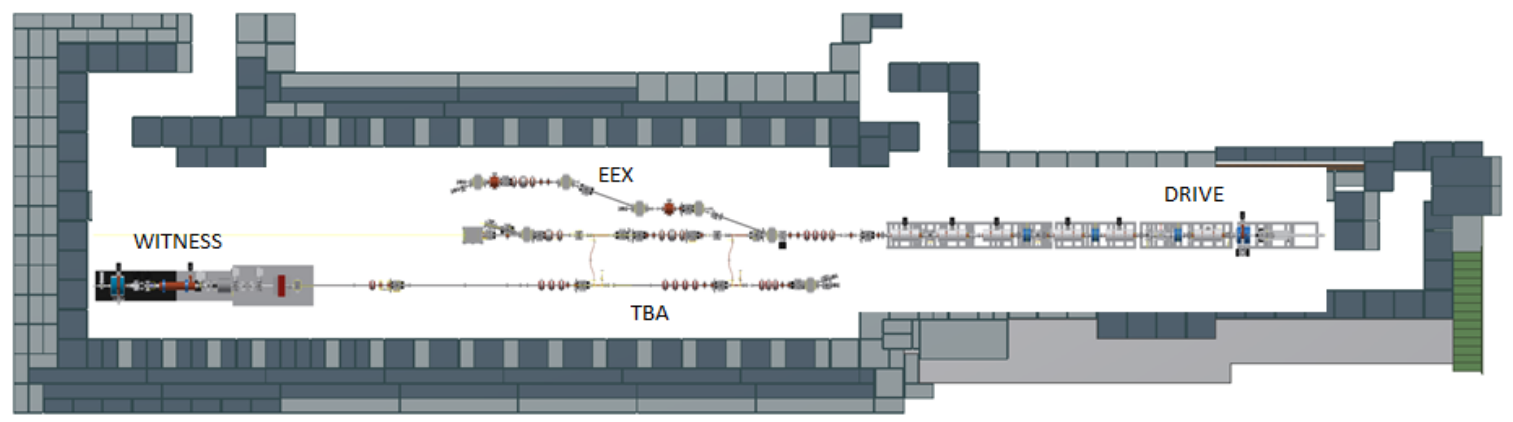
\includegraphics[width=\linewidth]{./images/bunker}
	\end{center}
	\caption{AWA Facility bunker and simplified TBA staging layout. 
		The drive beam line (right) supplies high charge bunch trains at \SI{70}{MeV}.
		The witness beam line (left) supplies a low charge single bunch at \SI{15}{MeV}. 
		CAD drawing of bunker courtesy of Scott Doran at AWA.}
	\label{fig:bunker}
\end{figure}
\begin{figure}
	\begin{center}
		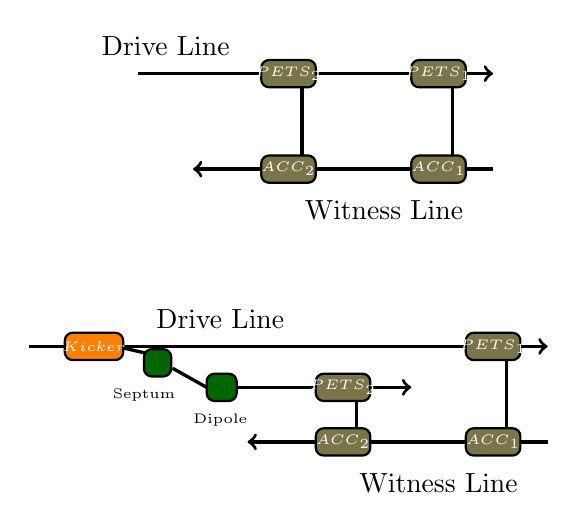
\begin{tikzpicture}[scale=\textwidth/35cm, text=black]
		\def \gunleft {-1.0}
\def \gunright {0.3}
\def \loneright {1.0}
\def \ltworight {2.0}
\def \lthreeright {3.0}
\def \lfourright {4.0}
\def \lfiveright {5.0}
\def \lsixright {6.0}
\def \quadone {7.3}
\def \quadfour{16}

%Full Staging
\draw[very thick, ->] (8,1) -- (27,1);

%Line between kicker and septum
\node[] at (15,2) {Drive Line};
\node[] at (23,-4) {Witness Line};
\draw[very thick] (\lsixright+5.2,1.0) -- (12.5,0.7);

%Kicker 
\draw[fill=orange,  thick, rounded corners =0.1cm] (\lsixright+3.3,0.5)rectangle ({\lsixright+0.84+4.6},1.5) node[pos=.5, white] {\tiny $Kicker$};
%Septum
\node[] at (12.2,-0.8) {\tiny Septum};
\draw[fill=black!60!green,  thick, rounded corners =0.1cm] (12.2,0.9)rectangle ({13.2},-0.1) node[pos=.5, white] {};
%Line between kicker and septum
\draw[very thick] (13.25,0.2) -- (14.5,-0.5);
%Dipole
\node[] at (15,-1.7) {\tiny Dipole};
\draw[fill=black!60!green, thick, rounded corners =0.1cm] (14.5,0.0)rectangle ({15.6},-1.0) node[pos=.5, white] {};
%Line between dipole and quads
\draw[very thick, ->] (15.6,-0.5) -- (22,-0.5);
%Witness
\draw[very thick, <-] (16,-2.5) -- (27,-2.5);
%Waveguide
\draw[very thick] (20,-0.5) -- (20,-3);
%Waveguide
\draw[very thick] (25.5,1.5) -- (25.5,-3);
%PETS2
\draw[fill=black!60!yellow,  thick, rounded corners =0.1cm] (18.5,0.0)rectangle (20.5,-1) node[pos=.5, white] {\tiny$\text{PETS}_2$};
%PETS1
\draw[fill=black!60!yellow,  thick, rounded corners =0.1cm] (24,1.5)rectangle (26,0.5) node[pos=.5, white] {\tiny$\text{PETS}_1$};
%ACC2
\draw[fill=black!60!yellow,  thick, rounded corners =0.1cm] (18.5,-2)rectangle (20.5,-3) node[pos=.5, white] {\tiny$\text{ACC}_2$};
%ACC1
\draw[fill=black!60!yellow,  thick, rounded corners =0.1cm] (24,-2)rectangle (26,-3) node[pos=.5, white] {\tiny$\text{ACC}_1$};



%Simplified Staging



\draw[very thick, ->] (12,11) -- (25,11);

%Line between kicker and septum
\node[] at (13,12) {Drive Line};
\node[] at (21,6) {Witness Line};

%Witness
\draw[very thick, <-] (14,10-2.5) -- (25,10-2.5);
%Waveguide
\draw[very thick] (18,11.5) -- (18,7);
%Waveguide
\draw[very thick] (23.5,11.5) -- (23.5,10-3);
%PETS2
\draw[fill=black!60!yellow,  thick, rounded corners =0.1cm] (16.5,11.5)rectangle (18.5,10.5) node[pos=.5, white] {\tiny$\text{PETS}_2$};
%PETS1
\draw[fill=black!60!yellow,  thick, rounded corners =0.1cm] (22,11.5)rectangle (24,10.5) node[pos=.5, white] {\tiny$\text{PETS}_1$};
%ACC2
\draw[fill=black!60!yellow,  thick, rounded corners =0.1cm] (16.5,8)rectangle (18.5,7) node[pos=.5, white] {\tiny$\text{ACC}_2$};
%ACC1
\draw[fill=black!60!yellow,  thick, rounded corners =0.1cm] (22,8)rectangle (24,7) node[pos=.5, white] {\tiny$\text{ACC}_1$};








		\end{tikzpicture}
	\end{center}
	\caption{Simplified drawing of the two staging schemes.
		No quadrupole elements are shown, and the arrows indicate what direction the beams travels.
		PETS stands for Power Extraction and Transfer Structure, and ACC stands for Accelerating structure. 
		The subscript on each structure refers to which stage the structures belong to (first or second). 
		In the simplified staging scheme the stages are not separated, meaning bunch train two travels
		through and loses energy in the first stage before reaching the second stage (top subfigure).
		This is prevented by separate beam lines in the full staging layout (bottom subfigure). }
	\label{fig:singlestage}
\end{figure}

Electron bunches in a photoinjector are created through the photoelectric effect. 
At the AWA, a pulsed UV laser is propagated through two relay lines of UV optics to either
the drive or witness gun. An in-vacuum mirror then directs the pulse to the photocathode.
Both beam lines must be operated simultaneously when the TBA experiments are run. This is accomplished by
splitting the original laser pulse into two pulses using a UV splitter on the 
ceiling of the bunker. One of the split pulses is sent (as is) to the witness beam line for one
bunch operation. The second pulse is sent to a UV multisplitter table, shown in 
Figure~\ref{fig:optics} where it is split into trains of various lengths. Eight pulses are 
used for TBA drive trains.

The RF photoinjector on the drive line uses a semiconducting
cesium telluride (CsTe) cathode, and is followed by a linear accelerator (linac). The
drive linac uses six copper cavities and four klystrons to accelerate the drive beam
to energies of $50-$\SI{70}{MeV}. The number of bunches generated from each 
laser pulse can vary from 1, 2, 4, 6, and 8 bunches. When multiple bunches
are generated, the grouping is called a bunch train. Generation of
these variable bunch trains is accomplished by splitting the pulsed
UV laser beam before it enters the gun and hits the cathode. The splitting
takes place in a complex network of UV optics located near the drive
gun. The optics setup is called a beam splitter, or mulitsplitter,
and trains are created at a rate of 0.5, 1, or \SI{2}{Hz}. 
This timing is the repetition rate of the machine. 
A simplified diagram of the laser pulse propagation is shown in Figure~\ref{fig:lasertiming}, 
and a picture of the AWA multisplitter table is shown in Figure~\ref{fig:optics}. 
Optimization of the UV optics was performed and is detailed in Section~\ref{sec:uvoptics}.  
\begin{figure}
	\centering
	\begin{tikzpicture}[every node/.style={anchor=south west,inner sep=0pt},x=1mm, y=1mm,]   
	\node (fig1) at (0,0)
	{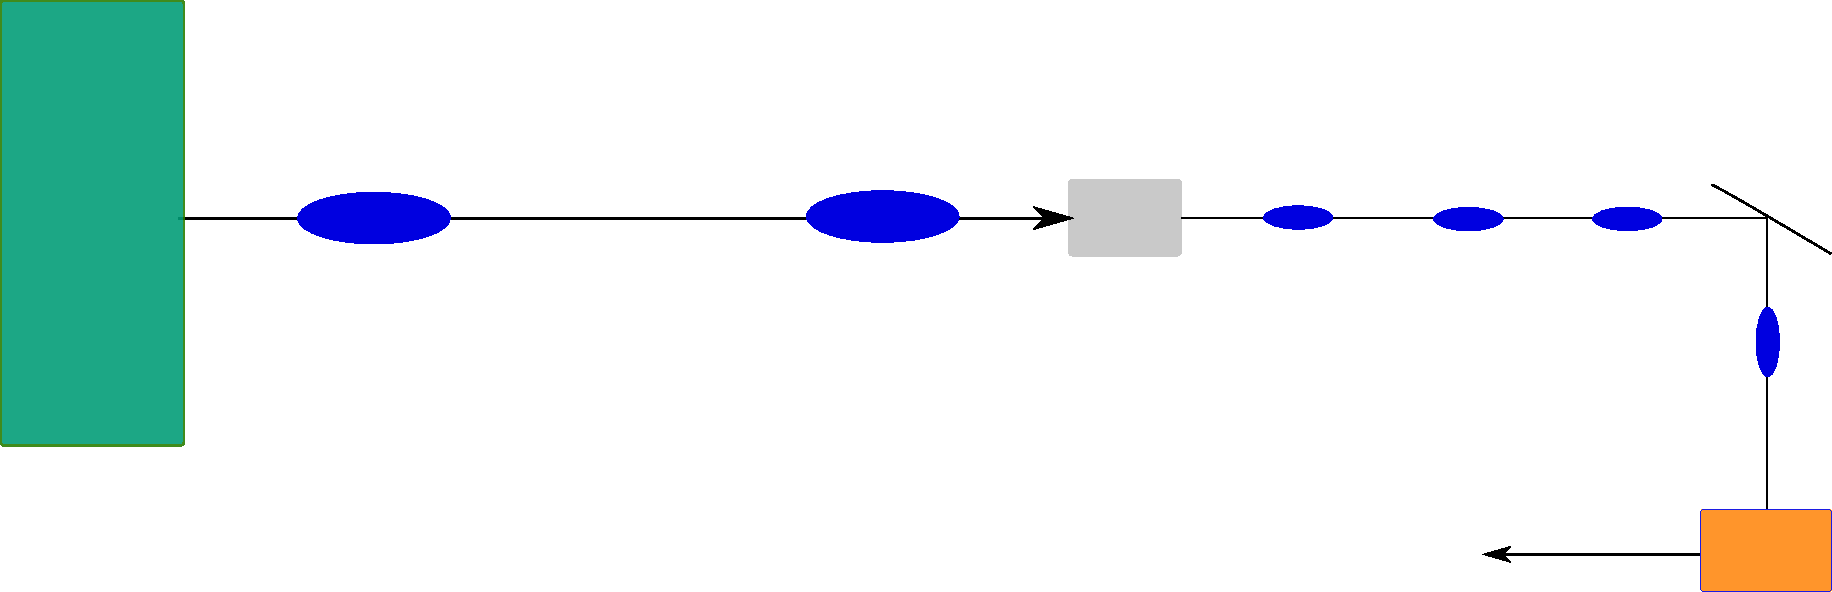
\includegraphics[width=0.85\textwidth]{images/laserpulsetrain}};
	\node[fill=white, inner sep=2pt] (txt2) at (-4,50) {Laser room};
	\node[fill=white, inner sep=2pt] (txt2) at (18,16) {Laser pulse};	
	\node[fill=white, inner sep=2pt] (txt2) at (87,16) {Laser pulse train};
	\node[fill=white, inner sep=2pt] (txt2) at (67,33) {Multisplitter};	
	\node[fill=white, inner sep=2pt] (txt2) at (125,30) {Mirror};	
	\node[fill=white, inner sep=2pt] (txt2) at (120,-6) {Gun};
	\end{tikzpicture}
	\caption{Simplified drawing of the laser pulse as it travels to the gun.
	The spacing of the laser pulses exiting the laser room is equal to the 
	repetition rate of the machine (0.5, 1, or \SI{2}{Hz}).
	When in the multisplitter, the original laser pulse is split into a pulse train of
	2, 4, 8, or 16 pulses. 
	The intensity of original laser pulse is equal to the sum of all members in the pulse train.
	The spacing in the pulse train is one period of the sinusoidal RF voltage supplied to the cavities,
	which is \SI{1.3}{GHz} (T=\SI{769}{ps}). }
	\label{fig:lasertiming}
\end{figure}
\begin{figure}%[h]
	\begin{center}
		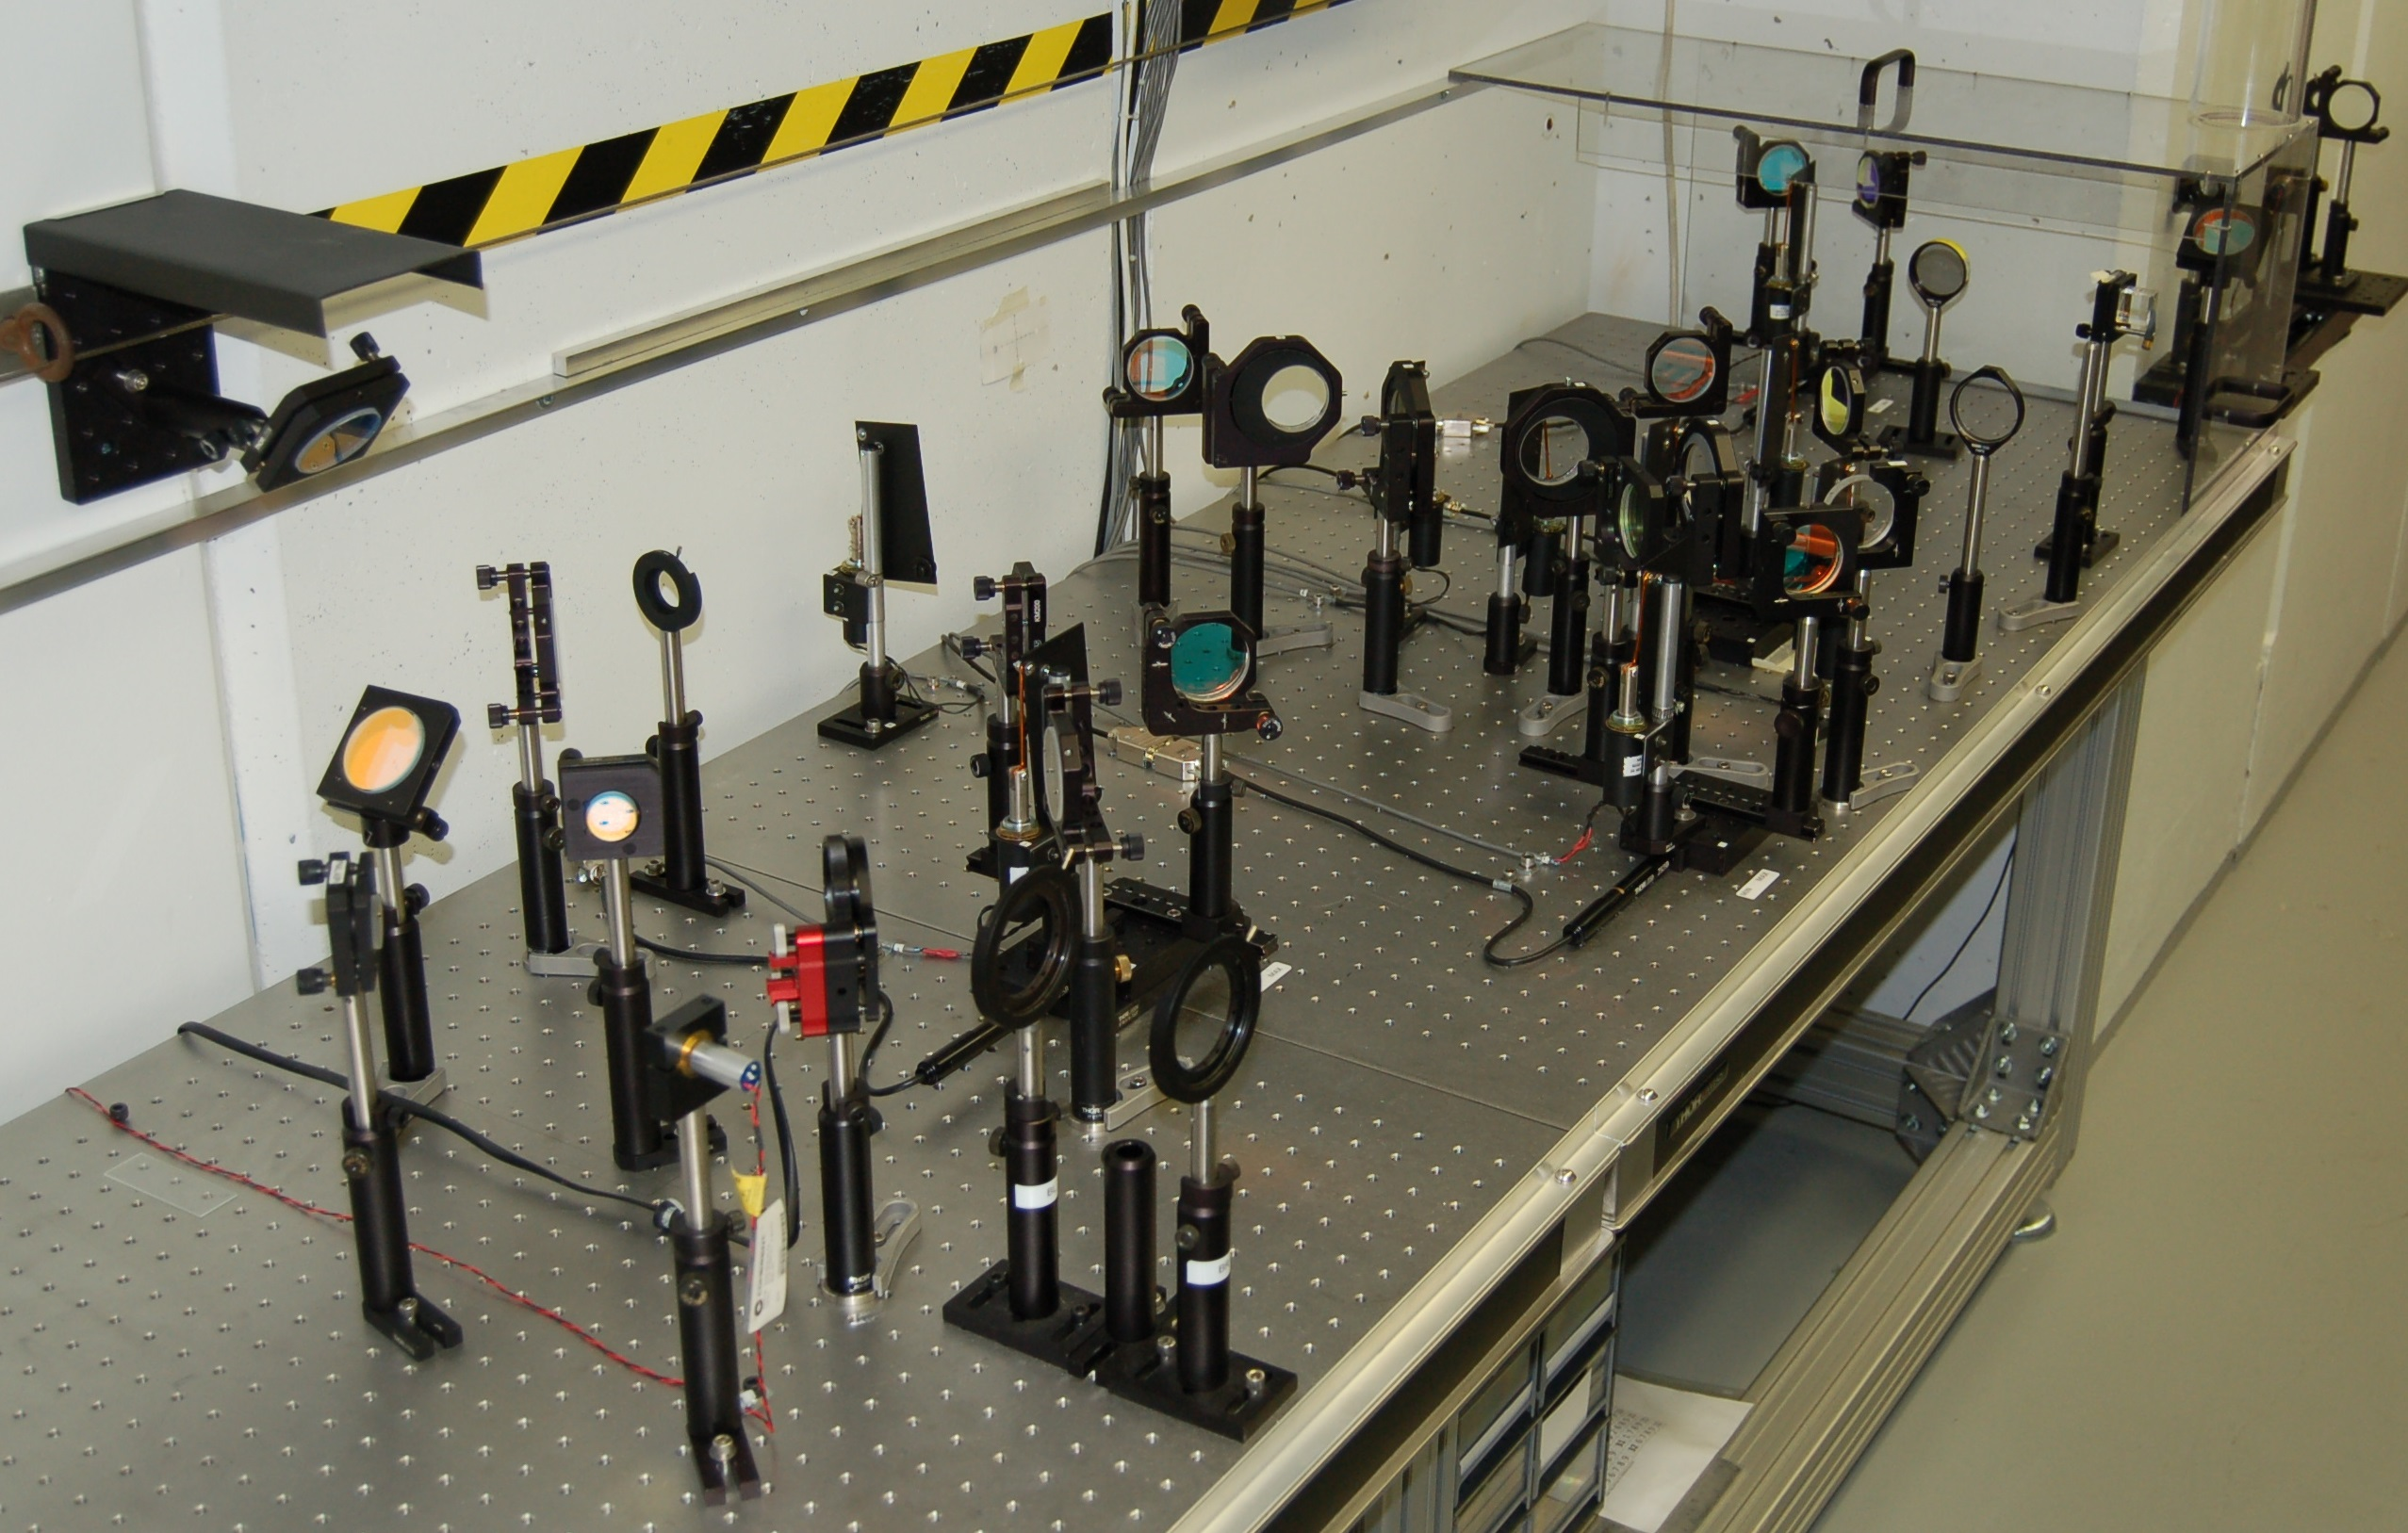
\includegraphics[width=0.7\textwidth]{images/multisplitter}
		\caption{UV multisplitter optics table.}\label{fig:optics}
	\end{center}
\end{figure}

The witness RF photoinjector, located on the left side of Figure~\ref{fig:bunker}, 
uses a magnesium cathode and the linac consists of one copper
accelerating cavity. Prior to the multisplitter table, shown in
Figure~\ref{fig:optics}, the laser pulse is split between the drive and witness side.
This setup allows only one bunch per pulse on the witness line. \\ 

%%%%%%%%%%%%%%%%%%%%%%%%%%%%%%%%%%%%%%%%%%%%%%%%%%%%%%%%%%%%%%%%%%%%%%%%%%%%%%%%%%%%%%%%%%%%
%%%%%%%%%%%%%%%%%%%%%%%%%%%%%%%%%%%%%%%%%%%%%%%%%%%%%%%%%%%%%%%%%%%%%%%%%%%%%%%%%%%%%%%%%%%%
\Section{Laser Pulse Train Improvement} 
\label{sec:uvoptics}
%%%%%%%%%%%%%%%%%%%%%%%%%%%%%%%%%%%%%%%%%%%%%%%%%%%%%%%%%%%%%%%%%%%%%%%%%%%%%%%%%%%%%%%%%%%%
%%%%%%%%%%%%%%%%%%%%%%%%%%%%%%%%%%%%%%%%%%%%%%%%%%%%%%%%%%%%%%%%%%%%%%%%%%%%%%%%%%%%%%%%%%%%

Initially some work had to be done for the production of a good quality  bunch train. 
Ideally, to extract maximum power from a series of bunches, 
each electron bunch should have the same amount of charge.  
Improving the laser pulse train intensity distribution improves the electron bunch charge distribution; 
which  helps produce an RF power pulse that is closer to uniform. 
The generated power depends on both the charge and shape of the bunch, as shown in Equation~\ref{eq:power1}. 
Several factors contribute to non-uniformity in the bunches. These include the cathode material
(i.e. slightly different QE along the surface), shot to shot noise in the laser pulse, 
distortion of laser pulses due to traveling through air, and the quality of the optics. 
The last is especially important in determining the intensity of each laser pulse in the train.  
Each splitter has a slightly different value for transmitted ($T$) and reflected ($R$) pulses. 

\Subsection{UV Optics} 
In order to generate the drive bunch trains needed for TBA, a UV laser pulse is split 
by five optical splitters into two trains of eight pulses. 
The optics setup is shown in Fig~\ref{fig:optics}. Optical delay lines (two mirrors) near each splitter 
separate pulses in space and time by extending the distance that each pulse travels. 
The length of each delay line is a multiple of the RF frequency, \SI{1.3}{GHz}. 
In other words, a separation of $1\lambda=$ \SI{23}{cm} (\SI{769}{ps}) between each UV pulse is created. 
This is done to synchronize the laser pulses with the RF voltage waveform supplied to the gun.
In order to achieve equally charged bunches, splitters with a perfect transmission 
to reflection ratio ($T/R = 50/50$) would be required.

\Subsection{UV Splitter Measurements} 
In reality, the complexity of optics coatings results in splitters that are not 
the ideal $T/R = 50/50$. This causes the intensity distribution in the 
laser pulse train to be non-uniform. 
The initially installed splitters were rated at a tolerance of $50\%\pm5\%$.
Measurements of the UV splitters were done to determine the $T/R$ (Transmission to Reflection) ratio for 
each splitter. The measurements took place in the laser room, close to the source of the laser.
The setup included two joule meters; one to measure the raw $T/R$ values and one to measure 
the background. Amplified Spontaneous Emission (ASE), 
is the main contributor to background shot to shot noise in the laser pulse,
and is known to drift with temperature and operating time. 
The ASE value was measured when each $T/R$ measurement was taken, then divided out of the $T/R$ 
measurements to prevent bias due to background drifts. 

Several configurations were tested this way: S-polarization, P-polarization, 
and laser incident on the back or front of the coating. 
Whether the laser pulse hit the front or back of the optic
had no measurable effect on the $T/R$ ratio. Polarization did have a significant effect on
the results. The AWA now monitors polarization orientation of all optics.  
Table~\ref{tab:reflection} shows the $\pm 5\%$ splitters ratio measurements. 
\begin{table}%[hbt]
	\begin{center}
		\caption{Average transmission and reflection measurements for original $\pm 5\%$ splitters.}
		\label{tab:reflection}
		\rowcolors{2}{blue!15}{white}   
		\begin{tabular}{ccc}
			\toprule
			\toprule
			%\rowcolor{blue!30} 
			\textbf{Splitter \#} & \textbf{Reflection \%}  & \textbf{Transmission \%} \\ 
			\midrule
			1 &  47  &  53   \\ %[3pt]
			2 &  45  &  55   \\ %[3pt]
			3 &  47  &  53   \\		 
			4 &  44  &  56	\\
			5 &  44  &  56   \\ 
			\bottomrule
		\end{tabular}	
	\end{center}
\end{table}
This caused an uneven laser intensity distribution, as the bunch intensity depends on the path 
it takes through the multisplitter optics. Pulses that were transmitted more than one
time could have significantly lower intensities than other bunches.  
Consider the path of laser pulse 4 as shown in Figure~\ref{fig:tikz}. 
The pulse is transmitted through splitters 1, 2, and 4, but is reflected by splitter 3.
\def \delayvertical {1.5}
\def \delayoneleft {7.5}
\def \delaytworight{15}
\def \mycenter{10.0}
\def \labels{6.5}
\def \sone {-0.5}
\def \stwo {\sone+1.5}
\def \sthree {\stwo+1.5}
\def \sfour {\sthree+1.5}
\def \buffer{-4.5}
\begin{figure*}%[h]
	\begin{center}		
		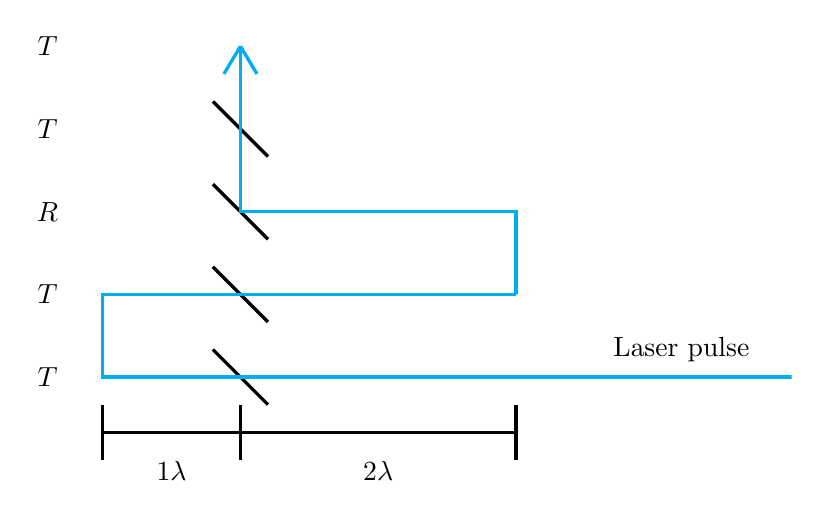
\begin{tikzpicture}[scale=0.7]
		%\node[] at (\labels, 5.5) {Behavior through splitter};
		\node[] at (\labels,6.0) {$T$};
		\node[] at (\labels,4.5) {$T$};
		\node[] at (\labels,3.0) {$R$};
		\node[] at (\labels,1.5) {$T$};
		\node[] at (\labels,0.0) {$T$};
		
		\draw[very thick] (10.5,\sone) -- (9.5,\sone+1); % Splitter 1
		\draw[very thick] (10.5,\stwo) -- (9.5,\stwo+1); % Splitter 2
		\draw[very thick] (10.5,\sthree) -- (9.5,\sthree+1); % Splitter 3
		\draw[very thick] (10.5,\sfour) -- (9.5,\sfour+1); % Splitter 4
		
		\draw[cyan, very thick] (\delayoneleft,0.0) -- (20.0,0.0) % Incoming pulse line
		to(\delayoneleft,0.0) -- (\delayoneleft,\delayvertical) % Delay Leg 1 (a)
		to(\delayoneleft,\delayvertical) -- (15,\delayvertical); % Pulse after delay 1
		
		\draw[cyan,very thick] (\mycenter,\delayvertical*2) -- (\delaytworight,\delayvertical*2)
		to(\delaytworight,\delayvertical) -- (\delaytworight,\delayvertical+1.5)
		to(\mycenter,\delayvertical*2) -- (\mycenter,\delayvertical*4);
		
		\draw[cyan, very thick] (9.7,5.5) -- (10.0,6.0); % arrow head left
		\draw[cyan, very thick] (10.0,6.0) -- (10.3,5.5); % arrow head right
		
		\node[] at (18,0.5) {Laser pulse};
		
		\node[] at (8.75,-1.7) {$1\lambda$};
		\draw[black, very thick] (\delayoneleft, -1) -- (\delaytworight, -1);
		\draw[black, very thick] (\delayoneleft, -1.5) -- (\delayoneleft, -0.5);
		\draw[black, very thick] (\mycenter, -1.5) -- (\mycenter, -0.5);
		
		\node[] at (12.5,-1.7) {$2\lambda$};
		\draw[black, very thick] (\delaytworight, 3.0+\buffer) -- (\delaytworight, 4.0+\buffer);
		
		\end{tikzpicture}
	\end{center} 
	\caption{Example of a laser pulse path through multisplitter. $T$ indicates when the laser pulse is 
		transmitted through the splitter, and $R$ stands for when the laser pulse is reflected by the splitter. 
		The operating wavelength is $\lambda = \SI{23}{cm}$. Bends are accomplished with two UV mirrors, 
		one at each corner of the delay line.}
	\label{fig:tikz}
\end{figure*}


Each splitter reduces the intensity of the pulse as a new pulse is generated. Expected intensities
can be predicted by using the measured $T$/$R$ values for each splitter. For example, using $T/R=55/45$,
in Fig~\ref{fig:tikz} the laser pulse is transmitted four times and reflected once: 
\begin{equation}\label{eq:i4}
I_4 =  T \cdot R \cdot T \cdot T \cdot T \cdot I_0 \approx 0.041 I_0.
\end{equation}
Therefore, this pulse would have a fairly high laser intensity, because it was transmitted multiple times. 
In the worst case, the laser pulse could be reflected ($45\%$) three times and transmitted ($55\%$) twice: 
\begin{equation}\label{eq:i6}
I_6 =  T \cdot R \cdot R \cdot R \cdot T \cdot  I_0 \approx 0.028 I_0.
\end{equation}
This pulse would have a lower intensity when compared to the pulse traveling the path described in Equation~\ref{eq:i4}.
These trends were reflected in the electron bunch trains generated in the gun.
As a result, it was necessary to investigate methods to improve the intensity distribution. 

\Subsection{New UV Splitters}
To improve the intensity distribution, splitters with a consistent tolerance of $50\%\pm3\%$ were purchased, 
installed, and the laser energy was measured again. The quality of the splitters was nearly
the same for each splitter, and the bias leaned toward reflection, $T/R \approx 47/53$. 
With the bias now reversed, 
the trend in intensity distribution was also reversed. The possibility of using a combination 
of splitters from the $\pm3\%$ and $\pm5\%$ sets was explored. 
Using a Python script to compare all possible combinations, it was determined that using only 
$\pm3\%$ splitters would result in the lowest variation in intensity. 

\Subsection{Train Intensity Measurements}
The train intensity for an eight-pulse laser train was measured using the $\pm5\%$ and $\pm3\%$ splitters.
A train of sixteen will be used for TBA experiments, but eight was chosen for these measurements to
simplify the experimental setup, and to reduce interruption to beam time 
runs which were using the four splitter setup. 
\begin{figure}
	\begin{center}
		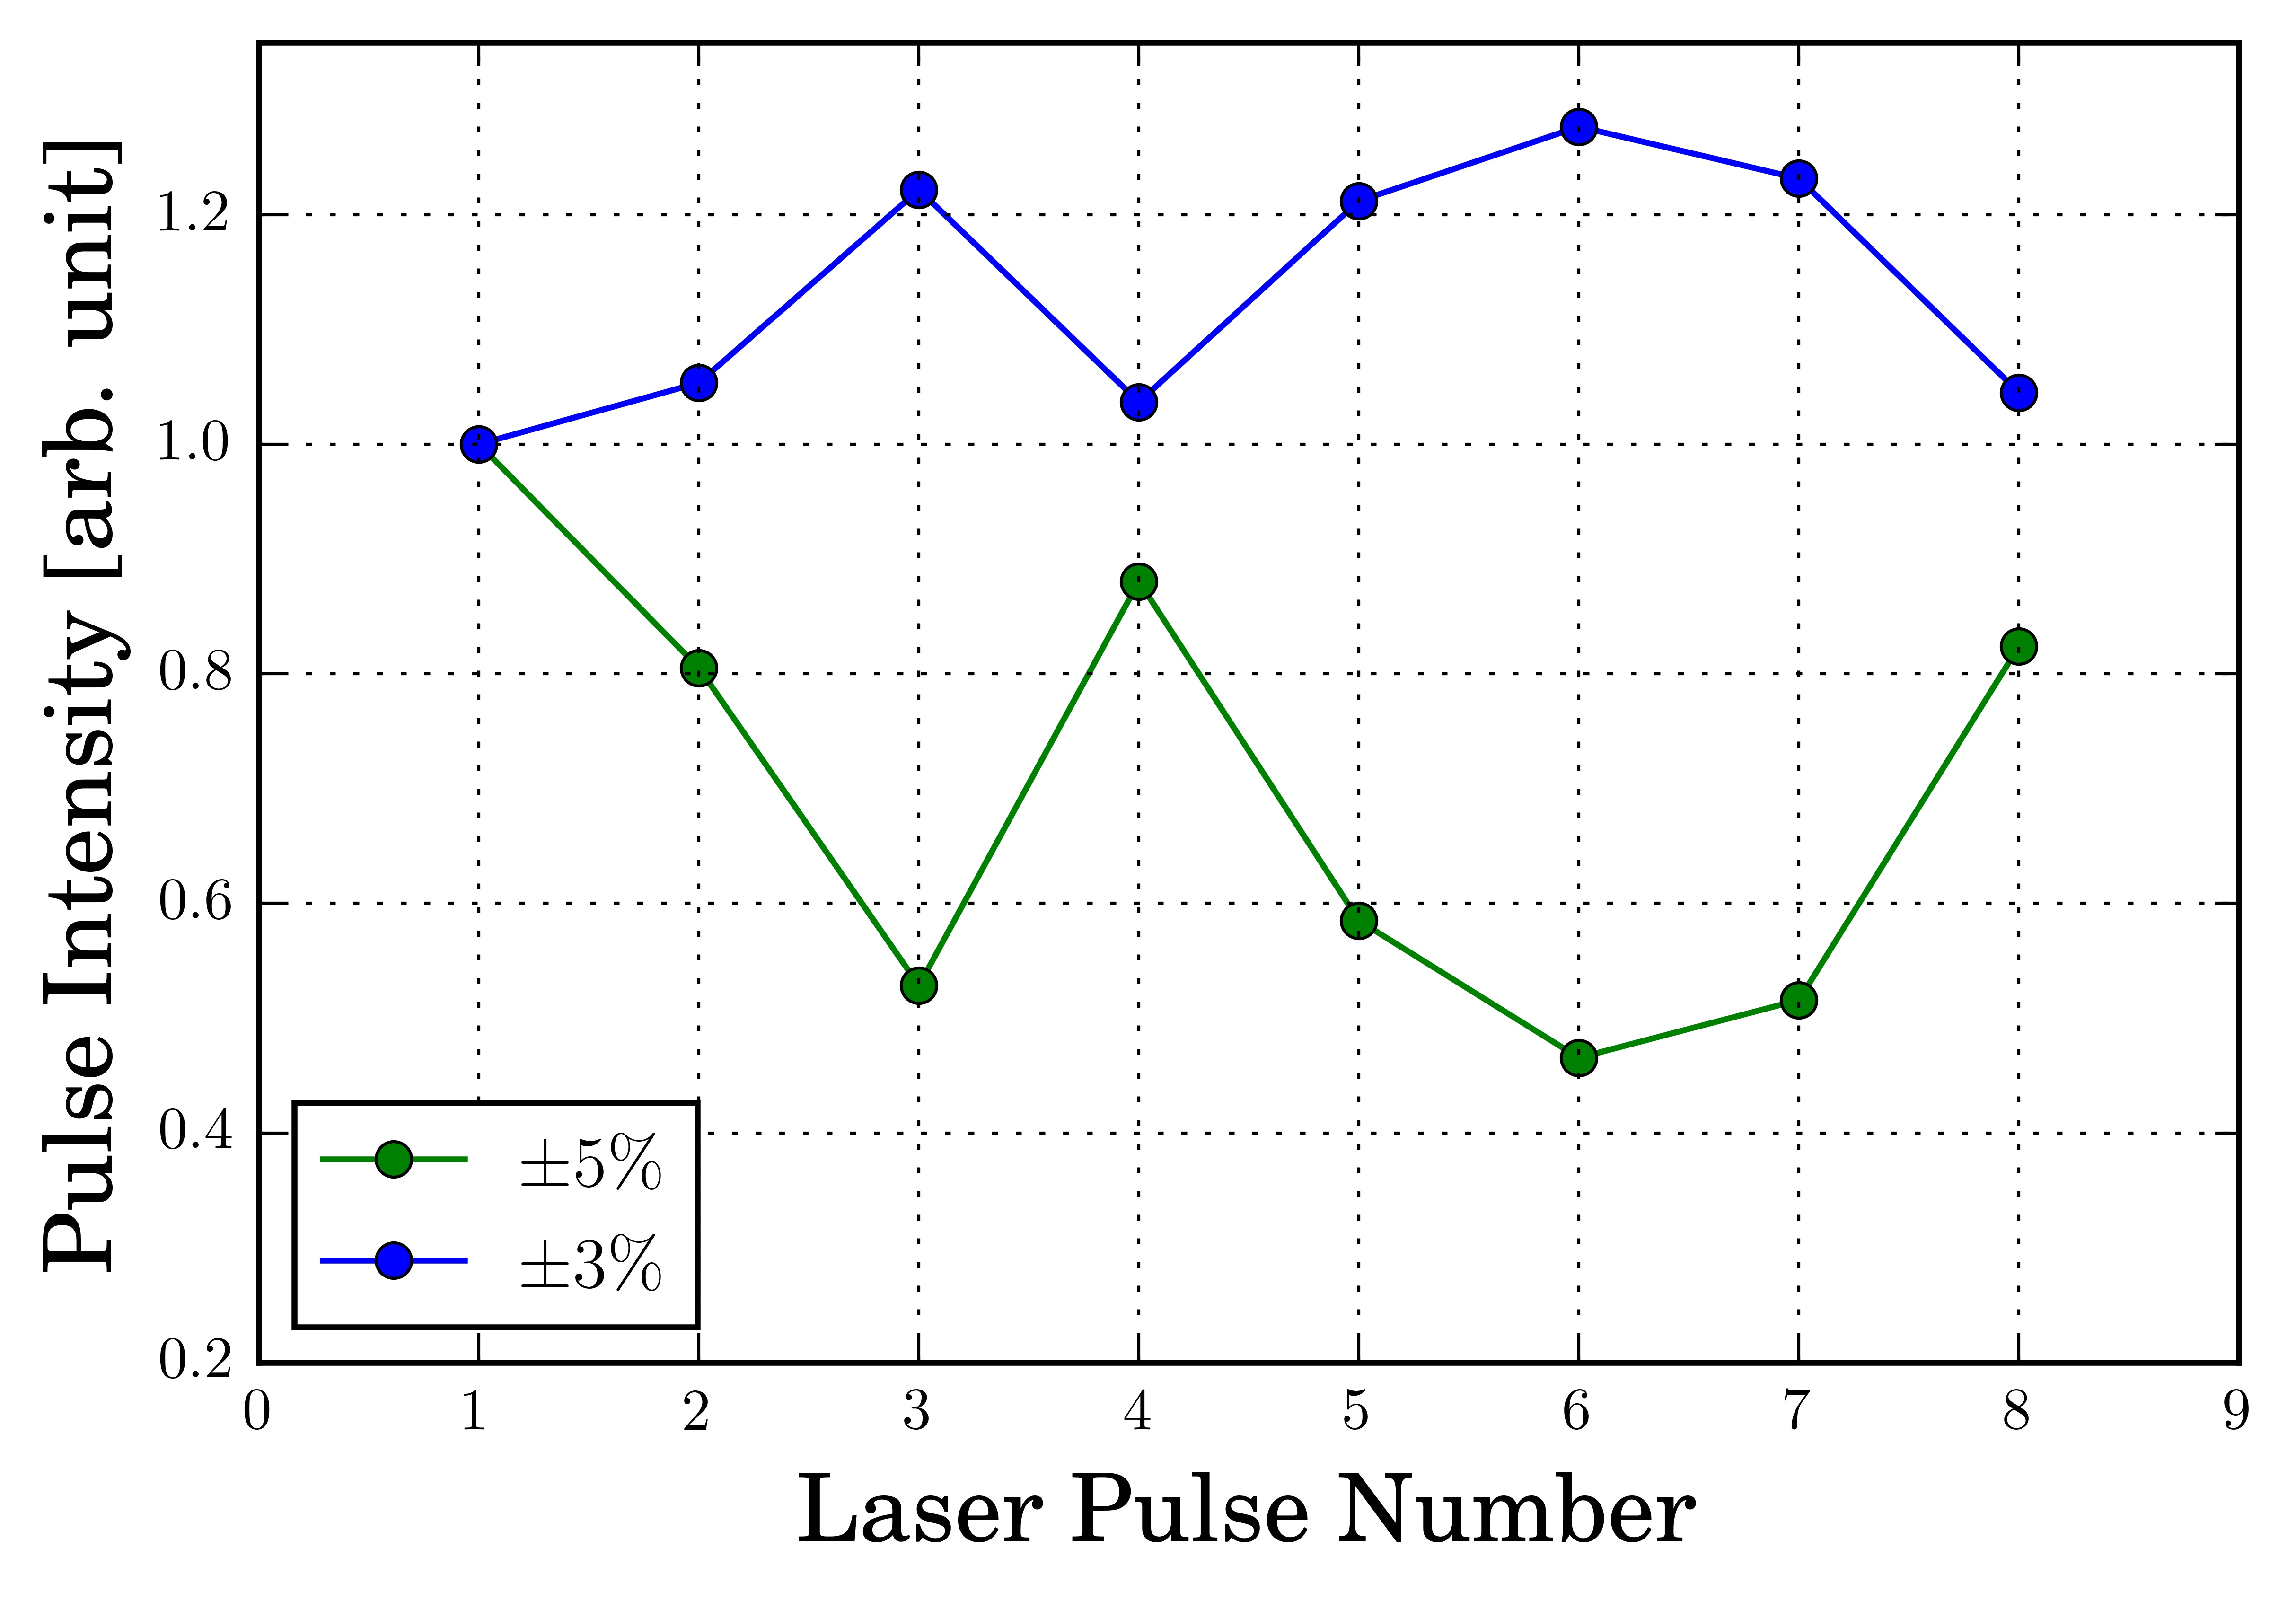
\includegraphics[width=0.75\textwidth]{images/splitter_improvement}
		\caption{Measurements of the laser pulse train intensity. The laser pulse number refers to 
			each pulse of light generated by the laser. These will respectively become electron bunch 1, 2, 3, and so on
			in the bunch train.}\label{fig:origtrain}
	\end{center}
\end{figure}
Equations~\ref{eq:i4} and~\ref{eq:i6} don't account for mirror losses in the delay legs, 
therefore a lower pulse intensity is expected in experimental measurements. The path of laser pulse 1 and
pulse 4 in the train can be described in the format of Equation~\ref{eq:i4}.
The number of splitters is four, and both pulses are transmitted three 
times and reflected once: 
\begin{align}
I_1 = R \cdot T \cdot T \cdot T \cdot I_0\, , \\
I_4 = T \cdot T \cdot R \cdot T \cdot I_0. 
\end{align}

With $\pm10\%$ mirror loss in the delay legs, laser pulse 1 and 4 are expected 
to be roughly the same intensity. This prediction matches the experimental measurements 
shown in Figure~\ref{fig:origtrain}. With the same 
logic, pulse 6 would have the largest deviation from pulse 1, as it is reflected 
three times and transmitted once in the four splitter setup. This expectation is also 
confirmed by the results in Figure~\ref{fig:origtrain}.  

While still not perfect, the laser pulse train is now more uniform.
Through the use of optics with tighter specifications and sorting of the optical elements, 
an improvement in laser pulse uniformity of 16.5\% was achieved.
This results in more uniform electron bunch trains, which means bunches 
of similar charge are delivered downstream. 
Since the power output in the PETS is a function of charge and bunch length, 
increased uniformity in the bunch train furthers the goals of demonstrating TBA 
by helping provide more consistent power output from the PETS.

%%%%%%%%%%%%%%%%%%%%%%%%%%%%%%%%%%%%%%%%%%%%%%%%%%%%%%%%%%%%%%%%%%%%%%%%%%%%%%%%%%%%%%%%%%%%
%%%%%%%%%%%%%%%%%%%%%%%%%%%%%%%%%%%%%%%%%%%%%%%%%%%%%%%%%%%%%%%%%%%%%%%%%%%%%%%%%%%%%%%%%%%%
\Section{RF Measurements}
%%%%%%%%%%%%%%%%%%%%%%%%%%%%%%%%%%%%%%%%%%%%%%%%%%%%%%%%%%%%%%%%%%%%%%%%%%%%%%%%%%%%%%%%%%%%
%%%%%%%%%%%%%%%%%%%%%%%%%%%%%%%%%%%%%%%%%%%%%%%%%%%%%%%%%%%%%%%%%%%%%%%%%%%%%%%%%%%%%%%%%%%%

In order to accurately simulate the RF fields in the linac cavities and gun on the drive and witness line, 
a set of detailed measurements were done to determine the power in each RF cavity.
These measurements are important, for several reasons. 
First, there are limited records at the AWA of these values in the past.
It is also important to know the fraction of power in each cavity 
with respect to the other cavities.
Ideally each cavity would be supplied the same amount of power, 
but as with all experimental hardware, the waveguide network is not ideal.
Two or more cavities are fed by one klystron which requires a network of 
power splitters and attenuators. If the power is not split evenly, the ratio 
of power delivered to each cavity may be different. 
The amount of attenuation in the subsequent waveguide after the spitter could
also be a source of power difference at the cavities.
 
In an effort to determine these differences, 
power measurements of the drive gun, and linac tanks 
two through six on the drive line were taken.
The next sections detail the calibration used during power measurements and the 
resulting values that informed simulations. 

\Subsection{Cable Calibration} \label{cablecal}
There is a significant length of cable that connects the cavities to the control room.
Since no cable is a perfect conductor, they do add attenuation to any signal propagated
and measured after the cables.
This attenuation needs to be accounted for so that the power measurements 
are accurate. The cable effects can be taken into account
by comparing a reference single supplied directly to the power meter
versus the reference single passed through the cables and then supplied to the power meter.
To do this comparison, a signal generator was placed in the tunnel, see Figure~\ref{fig:signalgenerator}. 
Then a signal was propagated to the control room where it was 
measured and compared to the original power measurement in the tunnel, see Figure~\ref{fig:tikzcalibration}. 
\begin{figure*}%[h]
	\begin{center}	
		\begin{circuitikz}[scale=0.7]
            \draw (0,0) to[csV=] (2,0);
            \node[align=center] at (0.8,2.0) {Signal \\ Generator};
            
			%Control room or power meter
			\def \leftside {3}
			\def \topbox {0.75}
			\def \botbox {-0.75}
			\draw (2.0, 0) -- (\leftside, 0);
			\draw[fill=white, ultra thick, rounded corners =0.1cm] (\leftside,\botbox)rectangle  
			({\leftside+3},\topbox) node[pos=0.5, align=center] {Meter};           
		\end{circuitikz}
    \end{center} 
\caption{Reference power reading was taken while power meter was directly connected to the 
signal generator. The resulting power was $P_s=\SI{-8.92}{dBm}$}
\label{fig:signalgenerator}
\end{figure*}
\def \delayvertical {1.5}
\iftrue
\begin{figure*}%[h]
	\begin{center}	
		\begin{circuitikz}[scale=0.7]
			
			\draw (0,0) to[csV=] (2,0);
			\node[align=center] at (0.8,2.0) {Signal \\ Generator};
			%Short blue RF cable 
			\node[] at (3.5,1) {$C_{1}$};
			\node[tlinestub] at (2,0){};
			\node[] at (3.5,-1) {};
			
			%Long RF cable
			\node[] at (7,1) {$C_{2}$};
			\node[tlinestub] at (5.5,0){};
			
			%Short yellow RF cable
			\node[] at (9.5,1) {$C_{3}$};
			\node[tlinestub] at (8.1,0){};
			%\draw[] (4.6,0) to[short,-] ++(1,0);
			\draw (4.6, 0) -- (5.6, 0);
			%10 dB attenuator
			\draw (10.7,0) to[R=$\SI{10}{dB}$, color=red] (14,0);
			
			%Control room or power meter
			\def \leftside {14}
			\def \topbox {0.75}
			\def \botbox {-0.75}
			%\draw (10.75, 0) -- (\leftside, 0);
			\draw[fill=white, ultra thick, rounded corners =0.1cm] (\leftside,\botbox)rectangle  
			({\leftside+3},\topbox) node[pos=0.5, align=center] {Meter};
		\end{circuitikz}
	\end{center} 
	\caption{Experimental setup when calibrating cables from the gun location to the control room. 
		Here $C_1$ is a short blue heliax, $C_2$ is a long heliax to the control room, 
		and $C_3$ is a short yellow heliax to the 6 GHz scope or power meter.}
	\label{fig:tikzcalibration}
\end{figure*}
\fi

The power reading in the control room was $P_c = \SI{-9.48}{dBm}$, and the power reading in 
the tunnel from the signal generator was $P_s = \SI{-8.92}{dBm}$, so the
attenuation is $\SI{0.56}{dB}$. 

\Subsection{Drive Gun Measurements}\label{gunenergy}
A power measurement was done to determine the accelerating gradient in the gun.
After the cable calibration, the setup was returned to typical operating conditions as 
shown in Figure~\ref{fig:tikzdrivegun}. This includes $\SI{53.2}{dB}$ from the gun pickup probe itself, a $\SI{36}{dB}$ additional attenuation from the pickup probe cable, followed by a long heliax to the 
control room. The signal is split in the control room with a mini-circuit ZFRSC-123-S+. 
Links to the specification sheets of all splitters used in this chapter can be found in Appendix~\ref{rf}.
One port is used for Low Level RF (LLRF) control, and the other port was connected to a short 
heliax, $C_3$, then to a $\SI{10}{dB}$ attenuator and finally to the 
power meter. Normally a load is placed at port two when a power meter is not connected. 
Next, the klystrons and phase shifters were set to supply 
maximum power to the gun, typical of TBA running conditions. 
\def \delayvertical {1.5}
\iftrue
\begin{figure*}%[h]
	\begin{center}		
		\begin{circuitikz}[scale=0.7]
			\def \leftside {17.0}
			\def \topbox {0.75}
			\def \botbox {-0.75}
			
			\node[] at (0.8,1.3) {Gun};
			\draw (0,0) to[csV=] (2,0);
			
			\def \gunright {2}
			%Attenuators
			%\node at (2, -0.50) {$P_1$};
			%\node at (5, -0.50) {$P_2$};
			
			\draw (\gunright,0) to[R=$\SI{53.2}{dB}$, color=red] (\gunright+2,0);
			\draw (\gunright+2.5,0) to[R=$\SI{36}{dB}$, color=red] (\gunright+4.5,0);
			\draw[] (\gunright+2.0,0) to[short,-] ++(0.5,0);
			%Long RF cable
			
			\node[] at (\gunright+6,1) {$C_{2}$};
			\node[tlinestub] at (\gunright+4.5,0){};
			\draw (9.0, 0) -- (10.0, 0);
			\draw[fill=white, ultra thick, rounded corners =0.1cm] (\gunright+8.0,\botbox)rectangle  
			%splitter
			({\gunright+11.0},\topbox) node[pos=0.5, align=center] {Splitter};
			\draw (11.5, 0.7) -- (11.5, 2);
			\node[] at (11.5, 2.5) {LLRF};
			
			%Short yellow RF cable
			\draw (13.0, 0) -- (13.5, 0);
			\node[] at (\gunright+13.0,1) {$C_{3}$};
			\node[tlinestub] at (\gunright+11.5,0){};
						
			%10 dB attenuator
			\draw (16.0, 0) -- (16.5, 0);
			\draw (\gunright+14.5,0) to[R=$\SI{10}{dB}$, color=red] (\gunright+16.5,0);
			
			%Control room or power meter
			\draw (18.5, 0) -- (\leftside+2, 0);
			\draw[fill=white, ultra thick, rounded corners =0.1cm] (\leftside+2,\botbox)rectangle  
			({\leftside+5},\topbox) node[pos=0.5, align=center] {Meter};
		\end{circuitikz}
	\end{center} 
	\caption{Experimental setup when measuring power from gun to control room. 
		Here $\SI{53.2}{dB}$ of attenuation is due to the gun probe itself, 
		$\SI{36}{dB}$ of additional attenuation is from the gun pickup probe cable in the tunnel, 
		$C_2$ is a long heliax to the control room. The $\SI{9.5}{dB}$  splitter sends half the signal to the   
		low level RF (LLRF) control system, and half to the power meter. 
		$C_3$ is a short yellow heliax that connects the meter to the splitter and on to the 6 GHz scope or power meter.}
	\label{fig:tikzdrivegun}
\end{figure*}
\fi

Using the setup in Figure~\ref{fig:tikzdrivegun}, the power meter measured  $P_{g} = \SI{-14.18}{dBm}$
in the control room. The attenuation must be accounted for 
to know the true power signal out of the gun: 
\begin{equation}
P_g =P_{meas} + A_{probe}+A_1 + C_2 + S + C_3 + A_2, 
\end{equation}
where $A_i$ represent attenuators, $C_i$ represent cable calibration numbers, 
and $S$ is the attenuation due to the splitter in the control room:
\begin{equation*}
\begin{aligned}
P_g \, \SI{}{[dBm]} = \\
\SI{53.2}{dB} + \SI{36}{dB} + \SI{0.56}{dB} \\
 + \SI{9.7}{dB}+ \SI{10}{dB} - \SI{9.07}{dBm} \\
 = \SI{100.39}{dBm}.
\end{aligned}
\end{equation*}

Then converting to a more convenient unit: 
\begin{equation}
P \, \SI{}{[dBm]} = 10 \cdot \log{\frac{P \, \SI{}{[mW]}}{\SI{1}{[mW]}}},
\end{equation}
\begin{equation} \label{eq:dbmtomw}
P \, \SI{}{[mW]} = \SI{1}{[mW]} \cdot 10^{\frac{P \, [\SI{}{dBm}]}{\SI{10}{}}},
\end{equation}
\begin{equation} 
P_2 = 10^{\SI{100.39}{dBm}} \cdot  \SI{1}{[mW]} = \SI{10.94}{MW}. 
\end{equation}


As described in Chapter 5 of E. Wisniewski's thesis~\cite{eric}, 
the power measurements can be related to the electric field 
based on the Superfish (SF)~\cite{superfish} model used to define the gun:
\begin{equation}
	\frac{E_{z \left(measured\right)}}{E_{z(SF)}} = \sqrt{\frac{P_{measured}}{P_{(SF)}}},
\end{equation}
\begin{equation}
	E_z = 1.86\sqrt{\frac{P_{measured}}{7.498\times10^-3}} = \SI{71}{MV/m}.
\end{equation}
Using the measurements above, this gives an estimate for the gradient in the gun.


\Subsection{Linac Cavity Measurements}
Next the power levels in the six linear accelerating (linac) cavities after the gun
were investigated. Information on the power ratio between cavities can 
guide simulation work. It is especially important to know if one cavity
has more or less power in the first two or three tanks, when the beam is at
lower energy and more susceptible to these differences.
Each are connected to the control room in the same way as the gun. 
The only differences are in the attenuation at the pickup probe and 
the splitter attenuation. The pickup probe attenuation is known only for cavities four and six.
Using the methods in section~\ref{gunenergy}, and the attenuation values,
the power in linac cavity four can be calculated:
\begin{table} %or [hbt] ?
	\caption{\label{tab:powerlinac} Power and attenuation values for the 
		linac cavities. Note that all cavities have an additional 
		\SI{33}{dB} attenuation added after the probe.
		The table is missing several probe attenuation values because the
		AWA currently has no record of these numbers.}
	\begin{center}
		\rowcolors{2}{blue!15}{white}
		\begin{tabular}{ccccc}	
			\toprule
			\toprule
			\textbf{Cavity} & \textbf{Probe Att.} & \textbf{Splitter Att.} & \textbf{Power Meter 1}  & \textbf{Power Meter 2} \\
			\midrule
			Gun & \SI{53.2}{dB}& $9.5 \pm \SI{0.3}{dB}$ & \SI{-14.18}{dBm} & \SI{-3.86}{dBm}  \\
			2 & --       & $9.5 \pm \SI{0.3}{dB}$ & \SI{-18.88}{dBm} & \SI{-9.6}{dBm}  \\
			3 & --       & $4.0 \pm \SI{1.0}{dB}$ & \SI{-12.24}{dBm} & \SI{-1.54}{dBm}  \\
			4 & \SI{61.95}{dB} & $9.5 \pm \SI{0.3}{dB}$ & \SI{-18.89}{dBm} & \SI{-10.11}{dBm}  \\
			5 & --       & $9.5 \pm \SI{0.3}{dB}$ & \SI{-17.76}{dBm} & \SI{-8.39}{dBm}  \\
			6 & \SI{61}{dB}    & $4.0 \pm \SI{1}{dB}$  & \SI{-14.32}{dBm} & \SI{-2.83}{dBm} \\
			\bottomrule
		\end{tabular}
	\end{center}
\end{table}
\begin{equation}
P_4 = \SI{-61.95}{dBm} + \SI{33}{dB} + \SI{0.56}{dB} + \SI{9.5}{dBm} +\SI{10}{dBm}.
\end{equation}

Four and six are the only cavities for which the gradients can be calculated, 
but the measurements still give an idea of which cavities are receiving more power.
For example, since linac cavity 2, 4, and 5 all share the same splitter, 
those measurements can be compared. It appears that cavity 5 is receiving about 
\SI{1}{dBm} more than 2 and 4. Comparing 3 and 6 indicates a larger discrepancy 
of \SI{2}{dBm}. Note, this comparison does assume the probe attenuations 
are not drastically different. 
With this information, simulations can be adjusted so that linac tanks 
3 and 5 receive slightly more power than the others. \\

\Section{Beam diagnostics}

There are several types of beam diagnostics that are used in 
TBA experiments at the AWA. They include instrumentation to measure beam size, energy, bunch length, 
and emittance. The first three diagnostics will be discussed in detail 
in the following sections. 

%%%%%%%%%%%%%%%%%%%%%%%%%%%%%%%%%%%%%%%%%%%%%%%%%%%%%%%%%%%%%%%%%%%%%%%%%%%%%%%%%%%%%%%%%%%%
%%%%%%%%%%%%%%%%%%%%%%%%%%%%%%%%%%%%%%%%%%%%%%%%%%%%%%%%%%%%%%%%%%%%%%%%%%%%%%%%%%%%%%%%%%%%
\Section{Energy Measurements} \label{sec:dipolecal}
%%%%%%%%%%%%%%%%%%%%%%%%%%%%%%%%%%%%%%%%%%%%%%%%%%%%%%%%%%%%%%%%%%%%%%%%%%%%%%%%%%%%%%%%%%%%
%%%%%%%%%%%%%%%%%%%%%%%%%%%%%%%%%%%%%%%%%%%%%%%%%%%%%%%%%%%%%%%%%%%%%%%%%%%%%%%%%%%%%%%%%%%

Energy measurements at the AWA are done with a dipole 
spectrometer magnet. The setup includes two Yttrium 
Aluminum Garnet (YAG) screens as shown in Figure~\ref{fig:spectrometer}.

\begin{figure*}%[h]
	\begin{center}		
		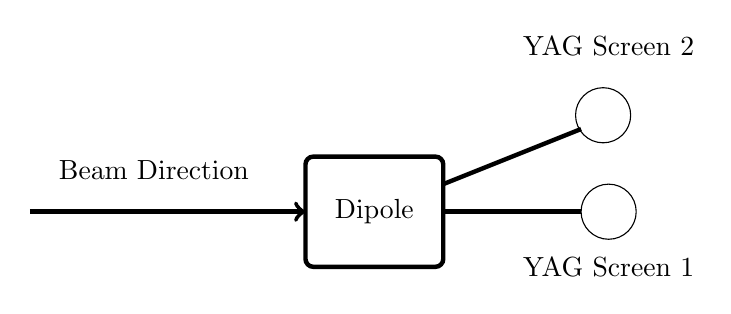
\begin{tikzpicture}[scale=0.7]
			
			\node[] at (2.25,0.75) {Beam Direction};
			\draw[ultra thick, ->] (0,0) -- (5.0, 0.0);
			
			\draw[fill=white, ultra thick, rounded corners =0.1cm] (5.0,1.0)rectangle  
			(7.5,-1.0) node[pos=0.5, align=center] {Dipole};
			
			\draw[ultra thick] (7.5, 0.0) -- (10.0, 0.0);
			\draw[ultra thick] (7.5, 0.5) -- (10.0, 1.5);
						
			\node[] at (10.5, 3) {YAG Screen 2};
			\draw (10.4,1.75) circle (0.5cm);
			
			\node[] at (10.5, -1.0) {YAG Screen 1};
			\draw (10.5,0) circle (0.5cm);
			
		\end{tikzpicture}
	\end{center} 
	\caption{Spectrometer setup in all cases at AWA.}
	\label{fig:spectrometer}
\end{figure*}

\Subsection{Energy Measurement Procedure}
Taking an energy measurement requires a beam trajectory
that is centered through the preceding quadrupole magnets. Otherwise, the beam 
may experience unintentional steering from the quadrupole magnets, and possibly excessive non-uniform fields 
if it enters the dipole off-axis. The centering is checked by powering the two 
quadrupoles before the dipole. The center is found by focusing 
in the x-direction, and then the y-direction. If the beam 
moves horizontally or vertically as it is being focused, 
the quadrupole is ``steering'', because the beam is entering the magnets off-axis.
Once the beam is centered through the quadrupoles on YAG screen 1, 
the dipole is then turned on to bend the beam.
The two YAG screens are positioned so that when the dipole is off, 
a centered beam will hit YAG screen 1. When the dipole is turned
on, its strength is adjusted until the beam appears at the center of YAG screen 2, corresponding to a 
$20^\circ$ bend. In this way, the dipole strength needed to center the beam on YAG screen 2 can 
then be used to determine the beam energy.

\Subsection{Energy Calculation}
Based on the procedure above, the current
supplied to the dipole is used to calculate the energy of the beam.
The current is determined by the number of ``counts''
keyed into the control system. A count-to-current conversion
was calculated based on the measurements shown in Table~\ref{tab:counts}. 
These measurements were taken independent of beam energy. 
Several current values were supplied to the dipole, and the corresponding
``counts'' in the control room were recorded.
\begin{table}
	\centering
	\caption{Counts to current data for the first dipole in the drive beam line.}
	\label{tab:counts}
        \rowcolors{2}{blue!15}{white}
	\begin{tabular}{c c} 
		\toprule
		\toprule
		Counts & Current [A] \\ [0.5ex] 
		\midrule
		1000 & 3.7 \\ 
		
		5000 & 18.8 \\
		
		10000 & 37.5 \\
		
		15000 & 56.3 \\
		\bottomrule
	\end{tabular}
\end{table}
After the current is determined, the magnetic field ($B$) is calculated: 
\begin{equation}
	\SI{}{B\,[T]} = (180.9708\cdot \SI{}{I\,[A]} - 7.2053)\cdot 10^{-4}.
	\label{eq:b}
\end{equation}
The slope and intercept were calculated using the measured $B$ vs. $I$ curve for the dipole.
\begin{figure*}
	\begin{center}		
		\begin{tikzpicture}[scale=1]
		\node (fig1) at (0,0)
		{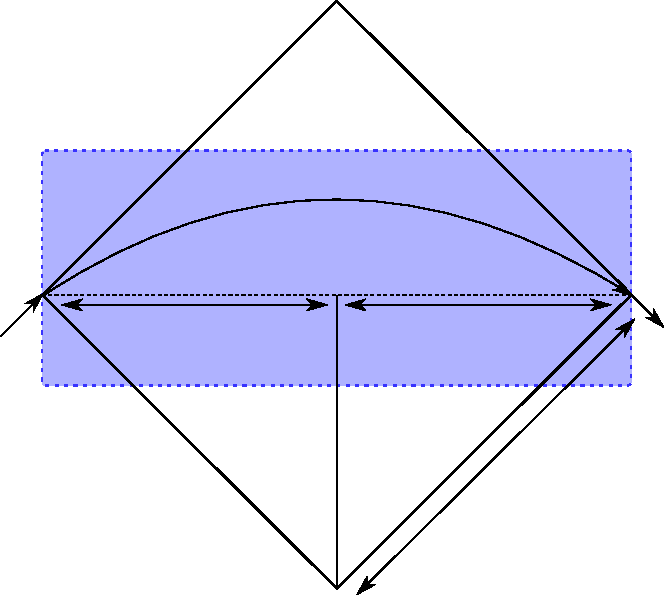
\includegraphics[width=0.5\textwidth]{./images/dipole_geometry}};
		\node[fill=white, inner sep=2pt] (txt2) at (-1.25,0.5) {$\frac{L}{2}$};
		\node[fill=white, inner sep=2pt] (txt2) at (-0.5,-2) {$\frac{\theta}{2}$};
		\node[fill=white, inner sep=2pt] (txt2) at (0.7,-2) {$\frac{\theta}{2}$};
		\node[fill=white, inner sep=2pt] (txt2) at (1.25,0.5) {$\frac{L}{2}$};
		\node[fill=white, inner sep=2pt] (txt2) at (2.5,-2) {$\rho$};
		\end{tikzpicture}
	\end{center} 
	\caption{Simplified drawing of the beam trajectory through a dipole with a uniform field. }
	\label{fig:dipole-geometry}
\end{figure*}

There are several geometric calculations that need to be done using the magnetic field value
before the energy can be calculated. The dipole geometry and variables used are shown in Figure~\ref{fig:dipole-geometry}.
The radius of curvature, $\rho$, can be calculated using the geometry shown in the figure, and 
will include the effective length of the dipole, L, and bending angle, $\theta$:
\begin{equation}
	\rho = \frac{L}{2\cdot \sin(\frac{\theta}{2})}.
	\label{eq:rho}
\end{equation}
Using $\rho$, and geometry, the x offset of the
beam after the dipole can be estimated: 
\begin{equation}
	\Delta x = \rho \left( 1- \cos\theta \right).
	\label{eq:xoff}
\end{equation}
Using the relationship, $B\rho$~\cite{Wiedemann},
the magnetic field in Tesla, B, and the beam momentum can be related: %\nrnote{\it check units}
\begin{equation}
	p\SI{}{\,\left[\frac{MeV}{c}\right]} = 0.2998\, B\cdot \rho \cdot 10^{3},
	\label{eq:pdipole}
\end{equation}
\begin{equation}
	\SI{}{E\,[MeV]} = \sqrt{0.511^2+(pc)^2}.
	\label{eq:energy}
\end{equation}

\Subsection{Dipole Example}
Since this calculation is used several times throughout the 
beam line for different magnets, a hard edge dipole example is shown 
to demonstrate how the above equations can be used to determine
the x offset after the magnet and the beam energy. 
The dipole length and bending angle are $L=\SI{0.2}{m}$, and $\theta=\SI{20}{^\circ}$. 
Using Equation~\ref{eq:rho}, 
the corresponding radius is $\rho = \SI{0.5759}{[m]}$. 
The offset, $\Delta x \approx \SI{34}{[mm]}$, can be calculated 
using Equation~\ref{eq:xoff}. This result was confirmed by a simulation in \verb|OPAL-t|.  

Now consider a second experimental case.
A beam of unknown energy passes through the dipole described above
with a bending angle of $20^\circ$. 
The current supplied to the magnet in order to achieve this bending angle is \SI{10}{A}.
Using Equation~\ref{eq:b}, the corresponding magnetic field is \SI{0.18}{T}.
Solving for the momentum with Equations~\ref{eq:pdipole}, and pulling the 
result into Equation~\ref{eq:energy}, 
the estimated energy of the beam is $\SI{49}{[MeV]}$.
This is how the the energy calculation is done for all measurements at the AWA.


%%%%%%%%%%%%%%%%%%%%%%%%%%%%%%%%%%%%%%%%%%%%%%%%%%%%%%%%%%%%%%%%%%%%%%%%%%%%%%%%
%%%%%%%%%%%%%%%%%%%%%%%%%%%%%%%%%%%%%%%%%%%%%%%%%%%%%%%%%%%%%%%%%%%%%%%%%%%%%%%%
\Section{Transverse Beam Size Measurements} \label{sec:beamsize}
%%%%%%%%%%%%%%%%%%%%%%%%%%%%%%%%%%%%%%%%%%%%%%%%%%%%%%%%%%%%%%%%%%%%%%%%%%%%%%%%
%%%%%%%%%%%%%%%%%%%%%%%%%%%%%%%%%%%%%%%%%%%%%%%%%%%%%%%%%%%%%%%%%%%%%%%%%%%%%%%%

Transverse beam size imaging and measurements are crucial to the 
operations at AWA. During experiments, these diagnostics give 
valuable information about the machine setup, help with alignment, 
and are used as a reference for tuning the beam line.
Basically, beam size measurements are the quickest way to evaluate the
optics configuration on the machine. 
These measurements are taken using YAG screens at multiple $z$ locations along the beam line.
The code used to produce all images in the following sections can be found at this git repository: 
\url{https://github.com/nneveu/imageProcessing}.
Note, all image routines referenced in this section can be found on the repository.

\Subsection{Capturing Images}
\begin{figure}
	\centering
	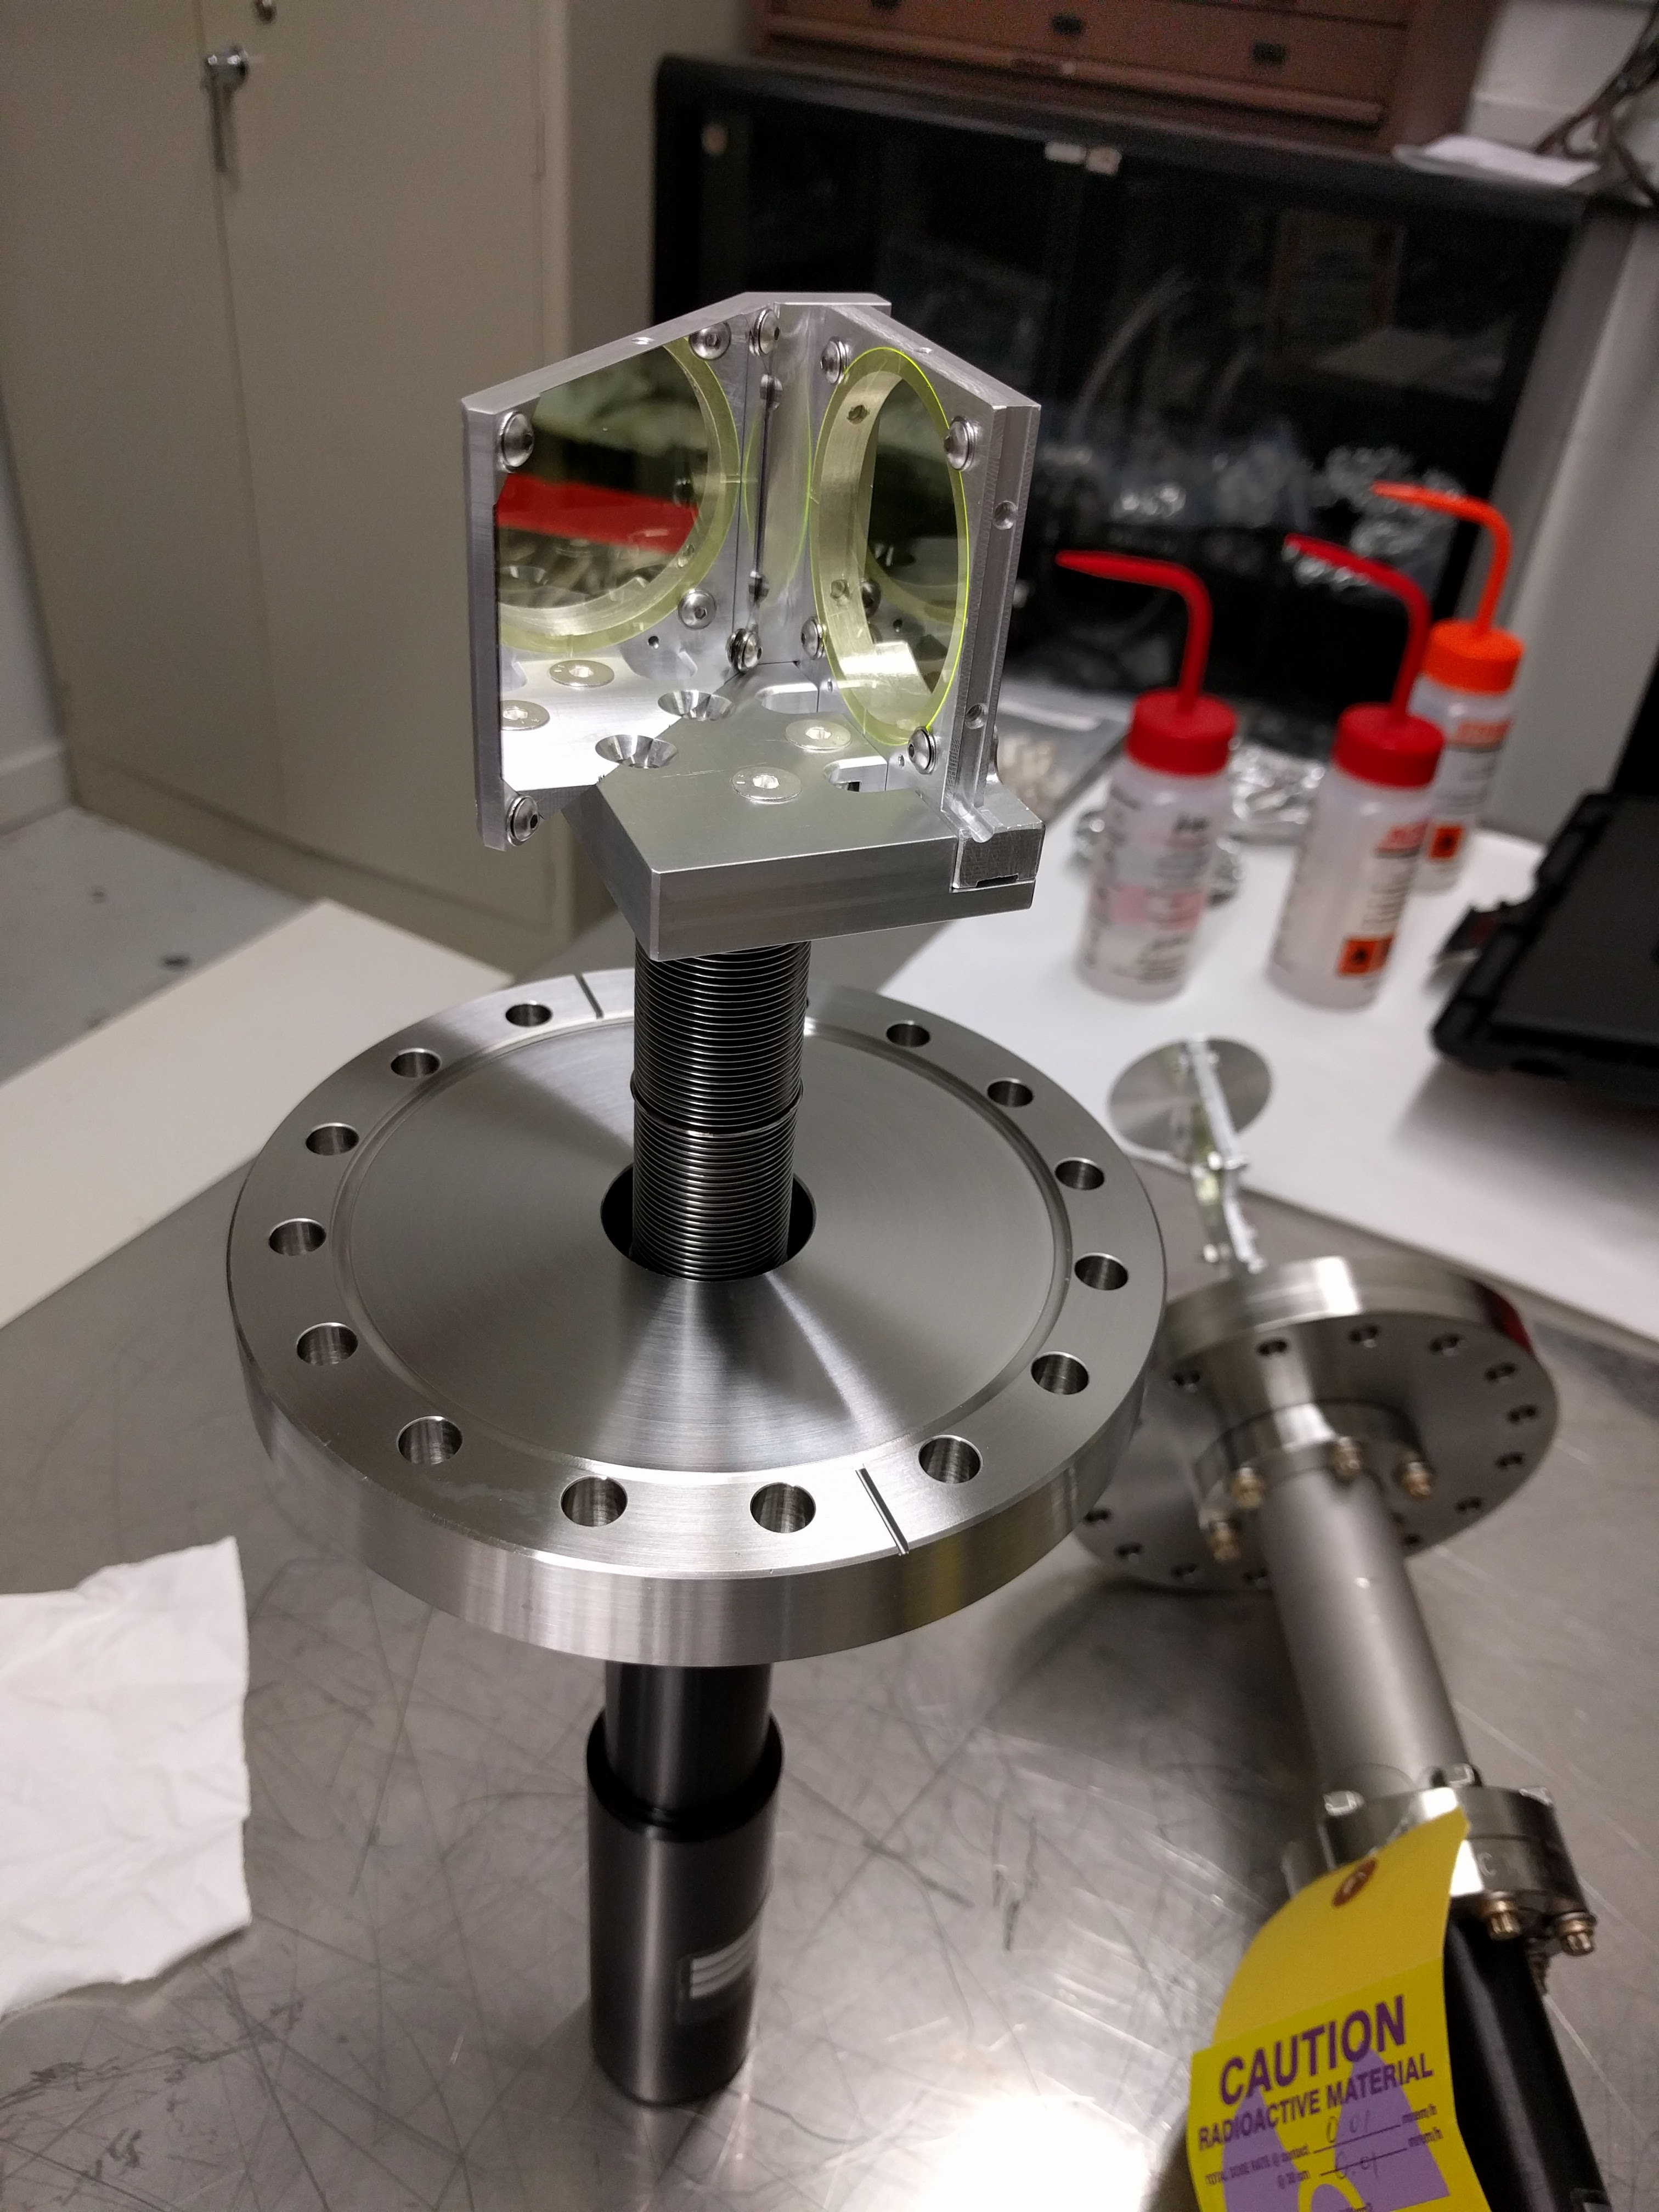
\includegraphics[width=0.75\textwidth]{images/YAG_screen}
	\label{fig:YAGscreen}
	\caption{Picture of a YAG screen diagnostic before installation in the beam line.
	The yellowish circle is the YAG screen and fluoresces when the beam hits it. 
	The mirror captures and directs the light to a camera positioned outside the vacuum chamber.}
\end{figure}
Raw YAG screen images can vary widely depending on the camera setup, charge, and 
light in the room. In some cases the edges of the metallic YAG holder
 are illuminated as shown in Figure~\ref{fig:yag-holder}.
Large amounts of dark current sometimes overlap with the electron beam as in Figure~\ref{fig:darkcurrent}, 
and on special occasions the image is fairly clean as in Figure~\ref{fig:clean}. 
The focal distance is different for every camera and depends on the physical camera and mirror
locations inside and outside of the vacuum chambers.
\begin{figure}	
	\centering
	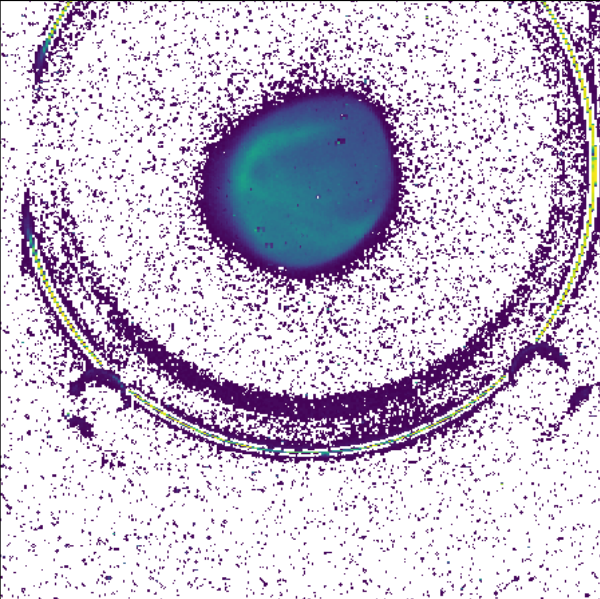
\includegraphics[width=0.5\textwidth]{images/yag-in-image}
	\caption{YAG screen image that is affected by the YAG holder fluorescing at an intensity that is greater than 
		background. The beam is too close to the holder to safely crop this area out.}
	\label{fig:yag-holder}
\end{figure}
\begin{figure}
	\centering
	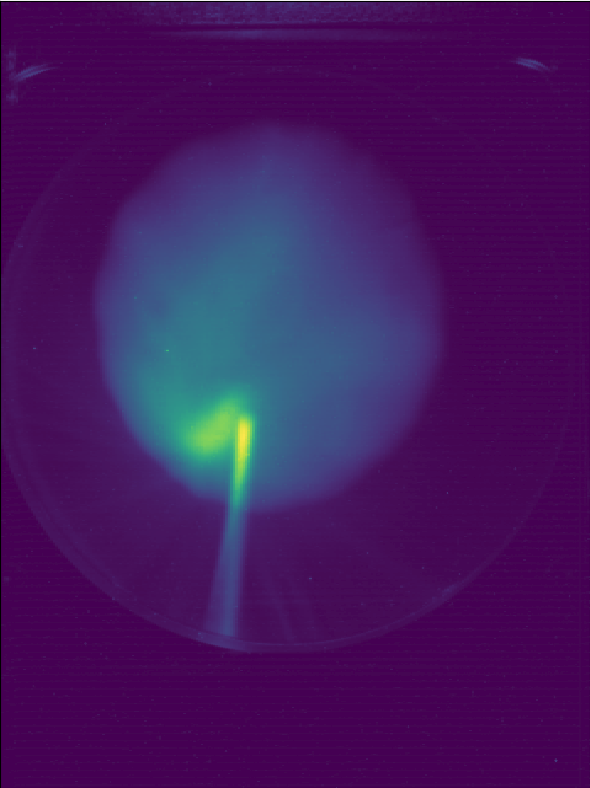
\includegraphics[width=0.45\textwidth]{images/darkcurrent}
	\caption{Yag screen image with dark current present. Background subtraction must take place to 
	analyze images with dark current.}
	\label{fig:darkcurrent}
\end{figure}	
\begin{figure}
	\centering
	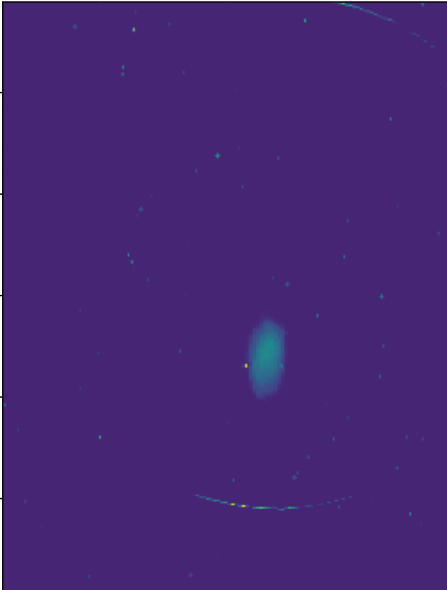
\includegraphics[width=0.5\textwidth]{images/cleanyag}
	\caption{Image where YAG holder light is far away enough from beam data that it can be safely cropped out.}
	\label{fig:clean}
\end{figure}

\Subsection{Post Processing Images}
A Python script was written to take beam images and calculate the beam size in x and y by finding the standard deviation, 
$\sigma_{x}$ and $\sigma_y$.  
This is done in a series of steps, and requires the availability of one or more images that can be used as a 
fiducial image. The fiducial image must clearly show the edges of the YAG screen so that a 
mm/pixel conversion can be calculated.
When dark current is present, an image of the dark current alone
(no photoemitted beam hitting the YAG screen) is necessary for background subtraction.
The following steps detail the post-processing from raw image to transverse beam size estimate.

\noindent\textbf{Step 1: Calculating the fiducial}
A fiducial image is used as a frame of reference. 
For the images at AWA, the YAG screen holder is used 
as the point of reference, because the radius is well-documented and known.
A good fiducial image should be well illuminated and have a clear view of the YAG holder 
edges as shown in Figure~\ref{fig:fiducial}.  
No beam is present in this image and the lights in the bunker are on.
\begin{figure}
	\centering
	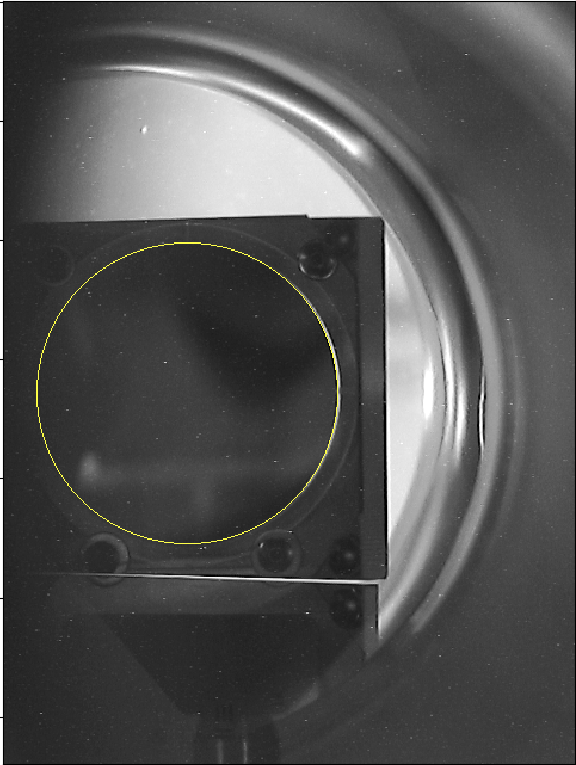
\includegraphics[width=0.5\textwidth]{images/YAG6_kicker_fiducial}
	\caption{Fiducial image taken of the sixth YAG screen on the drive line.
	The yellow circle is the resulting best fit using the Python script. }
        \label{fig:fiducial}
\end{figure}
After selection of an image, the \verb|circle_finder()| routine is used 
to fit a circle to the image and return the radius in pixels.
The fiducial can then be calculated,
\begin{equation}
	f = \frac{\SI{44.45}{mm}}{pixels}. 
\end{equation}
Once $f$ is known, it can be used to determine physical beam sizes.


\noindent\textbf{Step 2: Select on charge}
At the AWA, large charge fluctuations can occur when the laser intensity is not stable, 
this is especially true of high charge experiments, and less so for low charge operation.
The charge is a parameter that strongly impacts the beam size, 
therefore it is important to only compare beam images of similar charge value.
A reasonable range should be chosen for the experiment. 
Given a data set of 100 images and beam charge of roughly \SI{40}{nC}, 
a range of \SI{\pm0.5}{nC} has proven to be an acceptable cutoff.
The charge data is stored in a separate file, 
but saved at the same time as the image data. 
The charge data can be analyzed and used to return the indexes
that correspond to images of similar charges. 
This is done with the \verb|ict_charge()| and \verb|select_on_charge()| functions.
The charge is calculated by integrating the data using Simpson's rule.
The option exists to plot the ICT curve for visual inspection, an 
example is shown in Figure~\ref{fig:ict}
\begin{figure}
	\centering
	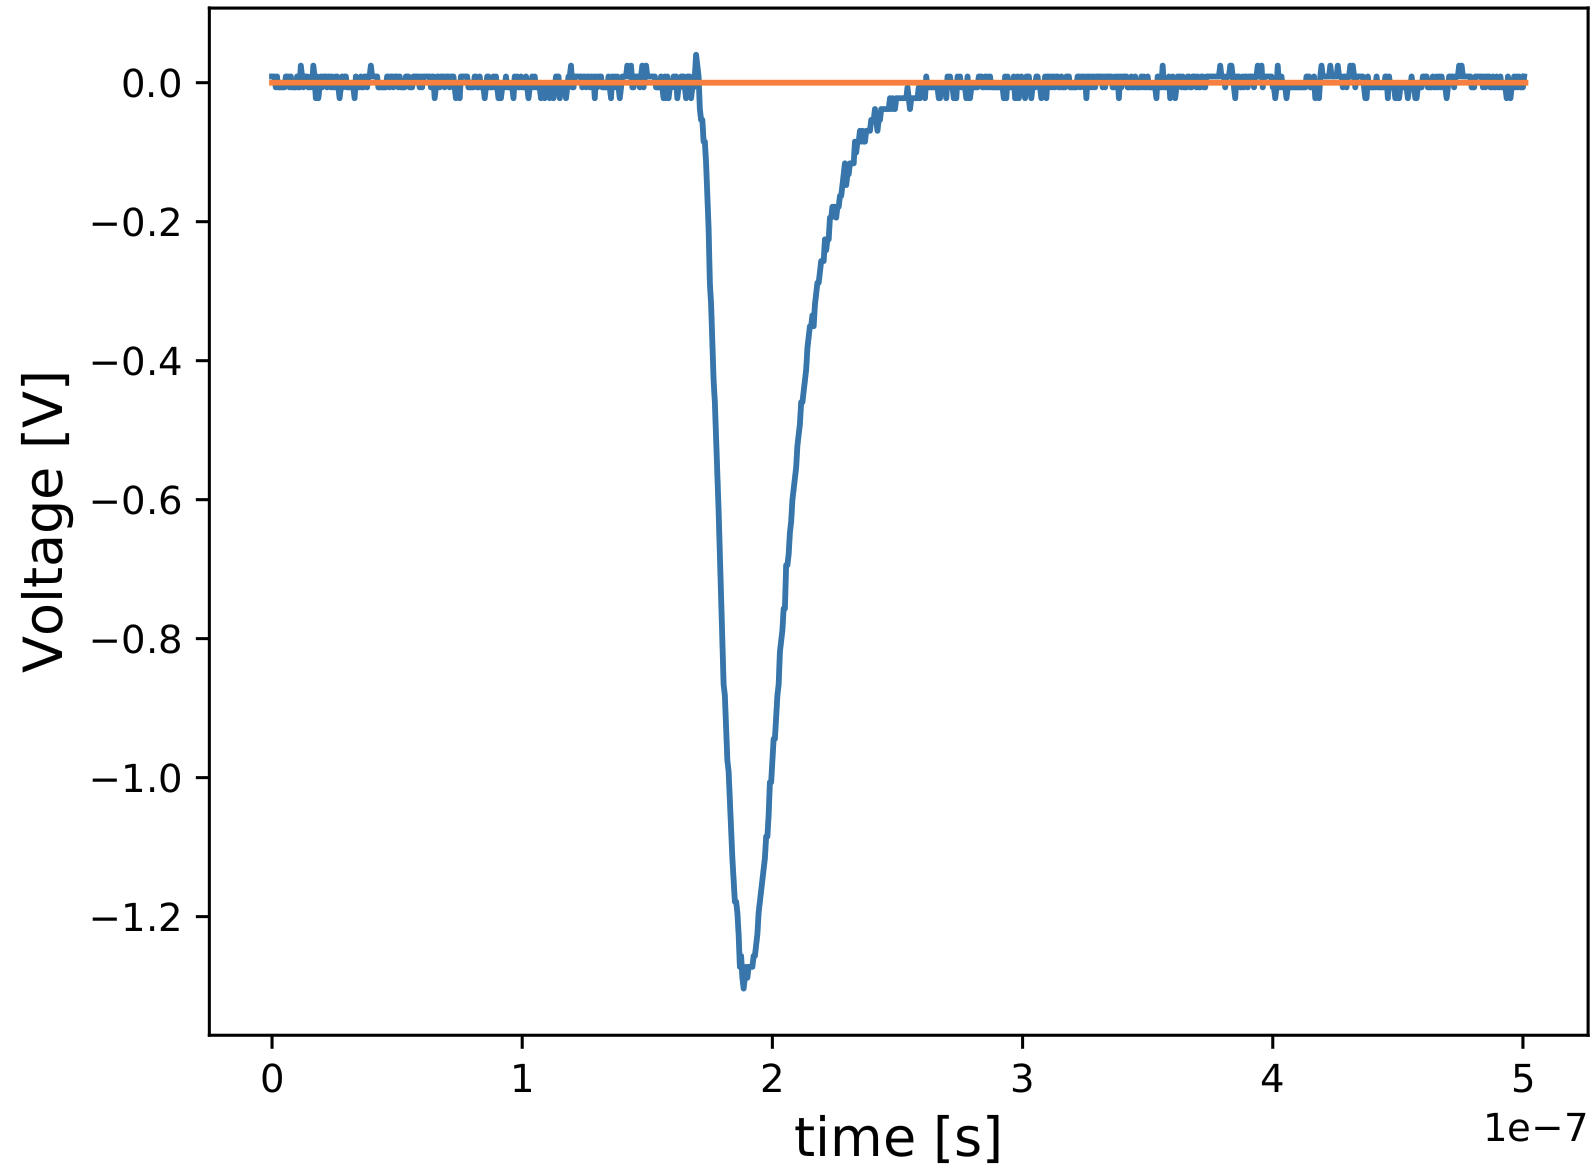
\includegraphics[width=0.75\textwidth]{images/ictcurve}
	\caption{Example of ICT data taken during an experiment. 
	One set of ICT data is taken for every image captured. 
	ICT and beam images are recorded simultaneously.}
	\label{fig:ict}
\end{figure}

\noindent\textbf{Step 3: Remove background intensity}
If dark current is present, it should be removed before determining beam sizes.
This can be done with a simple background subtraction if two appropriate images are available.
\begin{figure}
	\centering
	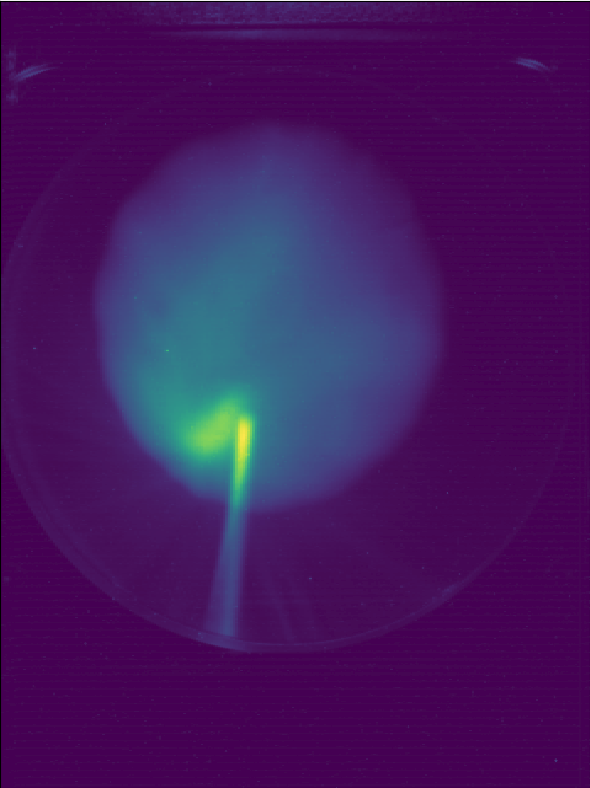
\includegraphics[width=0.3\textwidth]{images/darkcurrent}
	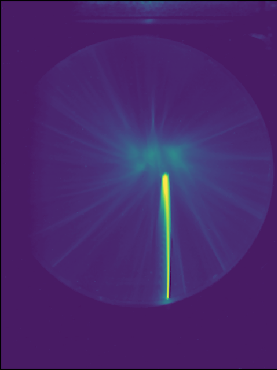
\includegraphics[width=0.3\textwidth]{images/backgroundonly}
	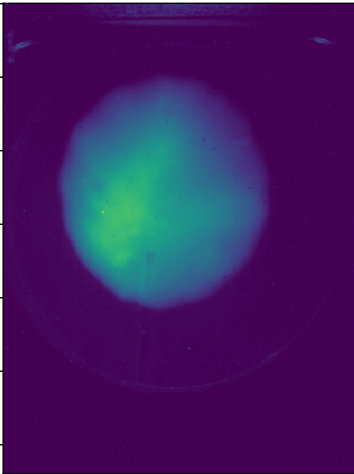
\includegraphics[width=0.3\textwidth]{images/background_cutout}%
	\caption{Example of an image with dark current. A background image is taken 
	when the beam is not present (middle picture). This is subtracted from the original beam image
	before calculating beam sizes.}
	\label{fig:backgroundsubtraction}
\end{figure}
First both the beam image and background image need to be loaded into 
arrays using the \verb|readimage()| function.
Next, a choice must be made on whether only one frame will be used 
as the background, or if averaging will be done. 
The dark current is a stable effect, but there can be some jitter.
Averaging can smooth jitter out in some cases, and can be done with 
the \verb|average_images()| routine. 
Next, a call to \verb|background_subtraction()| will do a simple pixel to 
pixel subtraction of the two images. Any negative pixel values are set to 0.
This case can occur when the background image is brighter than the beam image. 
For example, in Figure~\ref{fig:backgroundsubtraction} this would occur in regions 
where dark current is present, but no beam is (near YAG holder). 


\noindent\textbf{Step 4: Calculate x and y beam sizes}
With a fiducial, charge cut, and clean beam images, the beam size profiles can be generated.
This is done with a fitting model. Currently two options are implemented:
a pure Gaussian fit or a combination model that uses a Gaussian for 
the beam center and a linear fit for the tails (the edge of the beam).
This routine is called \verb|combo_model()| and uses methods from 
the \verb|lmfit| Python package.
This function returns beam sizes for every image and 
a correlation coefficient ($R$), as a measure of how well the fit matches the data. 
A plot is also made for each image, showing the data overlaid with 
the resulting fit, as shown in in Figure~\ref{fig:combo}.  
\begin{figure}
	\centering
	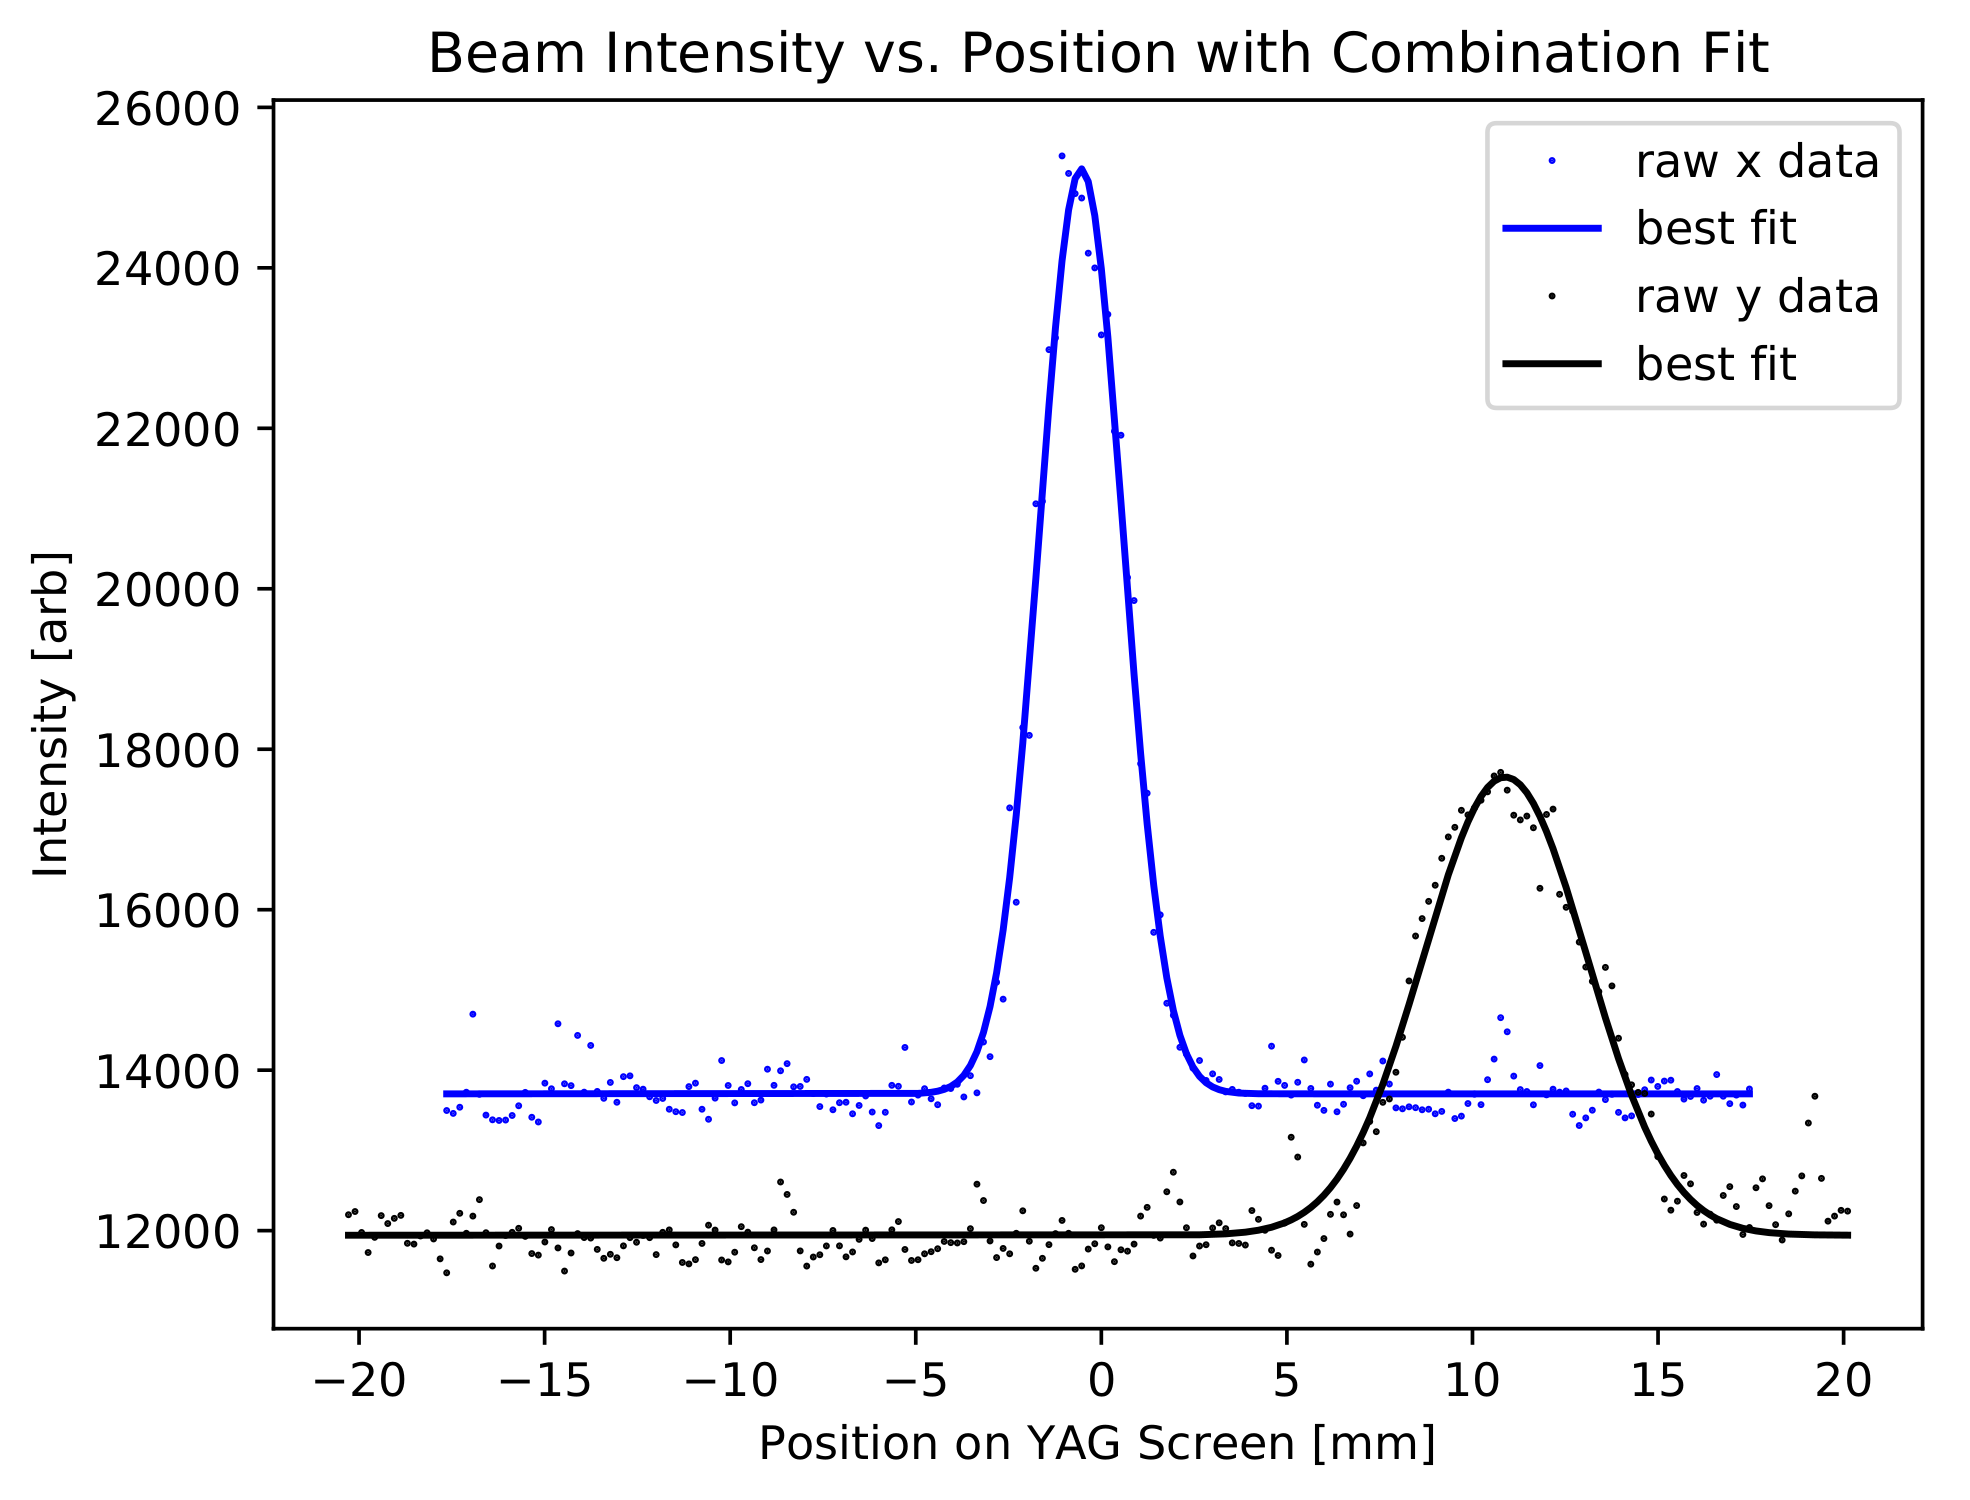
\includegraphics[width=0.75\textwidth]{images/combomodel}
	\caption{Beam profile fit overlaid on data. 
		The fitted curve is used to estimate the beam size.
	The data is not centered on zero because the beam was not centered on the YAG screen.
	This offset does not effect the beam size calculation, as only the fit is considered.}
\label{fig:combo}
\end{figure}

\noindent\textbf{Step 5: Add profile and dimensions to display image}
While the data in Step~4 is mostly numerical, it is helpful to 
display the beam profiles alongside the beam image. 
This can be done with \verb|add_dist_to_image()|. 
Both x and y projections are added to each axis, and give a visual representation of the beam size. 
The fiducial is needed for this step in order to add physical dimension to the image.
\begin{figure}
	\centering
	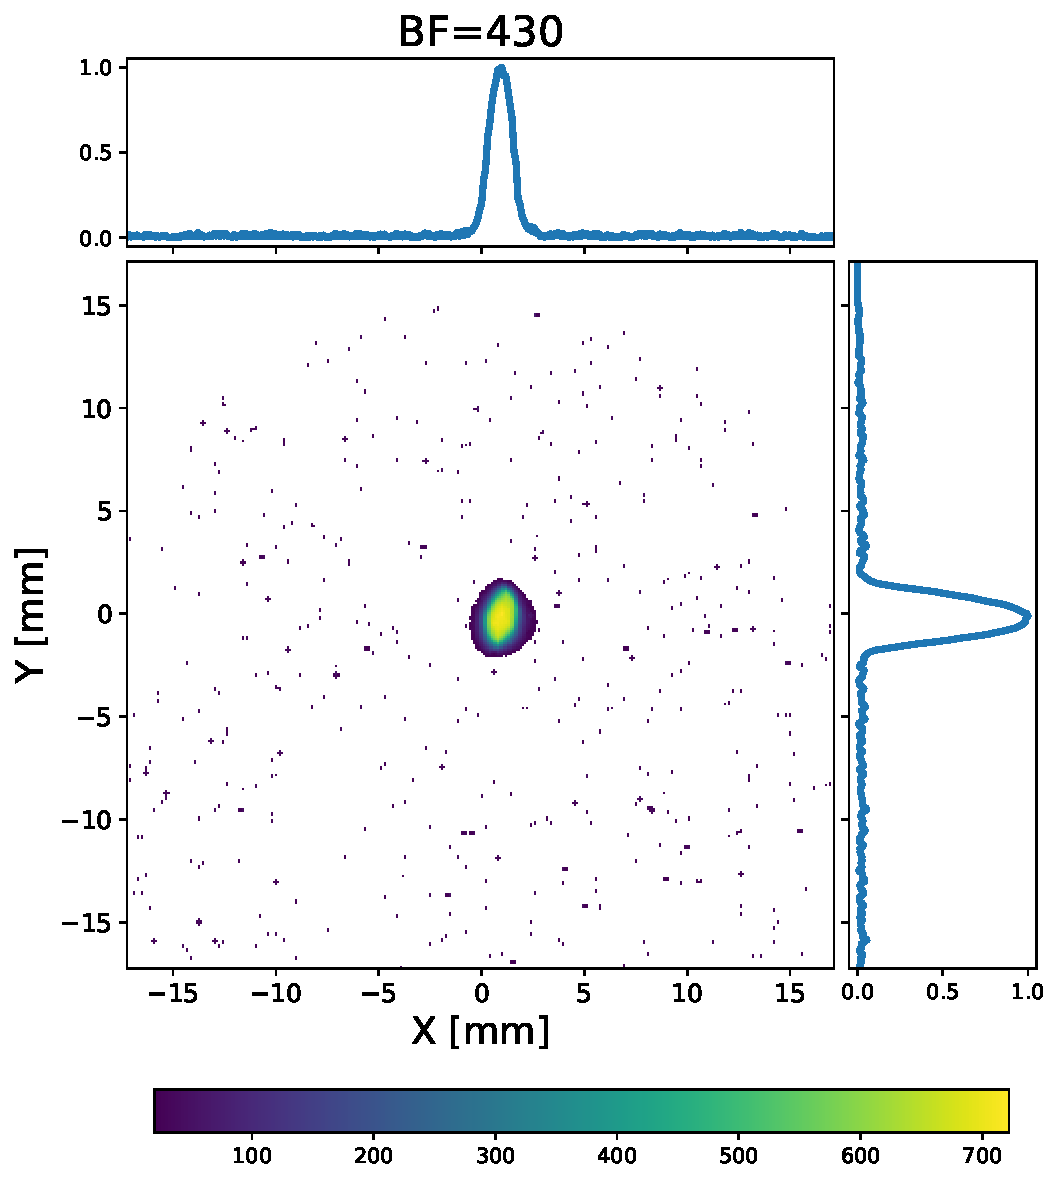
\includegraphics[width=0.5\textwidth]{images/yag1_1nC_M260_BF430}
	\caption{Average beam image with profile distribution.
	The speckled background is caused by background x-rays that are 
	generated when the accelerator is running.}
\end{figure}

\Section{Solenoid Scans}

Using the data analysis techniques in the previous section, 
solenoid scans were done to pin down discrepancies between 
simulations and experimental beam sizes. 
This method was used because of the simplicity of the experimental 
setup.
The data was taken at the first YAG screen in the beam line.
The only elements before this YAG screen are the gun, two solenoids, 
and one linac cavity. 
Scans were done at low charge (\SI{1}{nC}) and high charge (\SI{40}{nC}) see Figure~\ref{fig:solscan}. 
When post-processing the data, the beam sizes were smaller than expected.
There were two possible sources of this error. 
The matching solenoid field could be higher than expected, i.e. stronger focusing.
Or the gun gradient could be lower than expected, resulting in a lower energy 
beam that would be focused more strongly by the solenoid field.
This work motivated a new measurement of the solenoid field strength when 
the cathode was changed. It was determined that the field is behaving as expected, 
which indicates the gun gradient is lower than previously estimated.
\begin{figure}
	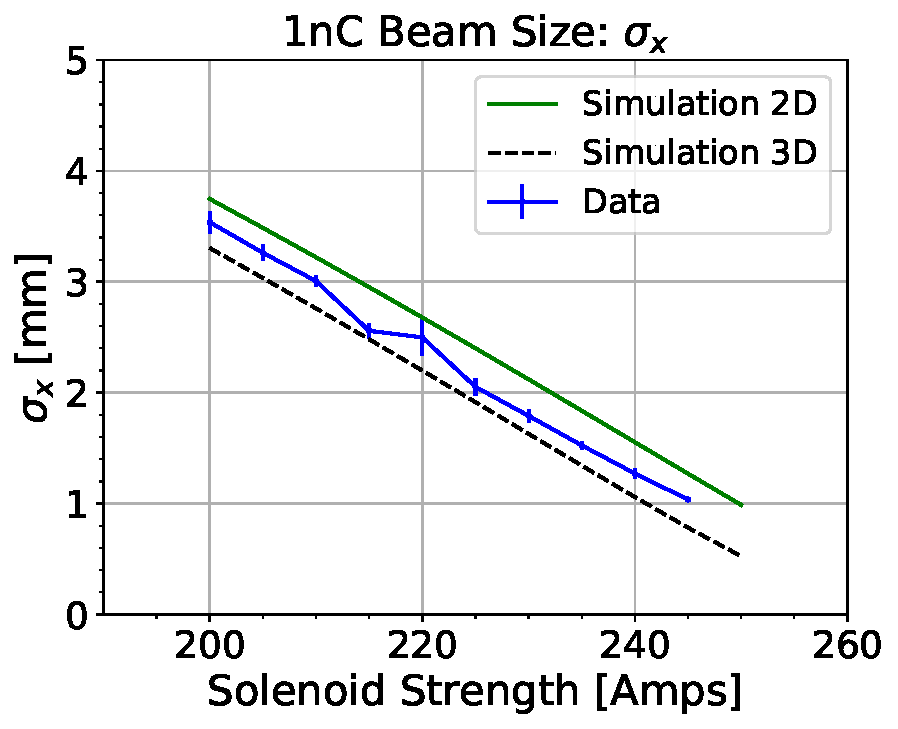
\includegraphics[width=0.45\textwidth]{images/xbeamsizes_low_charge_sol_scan_11-02-2017}%
	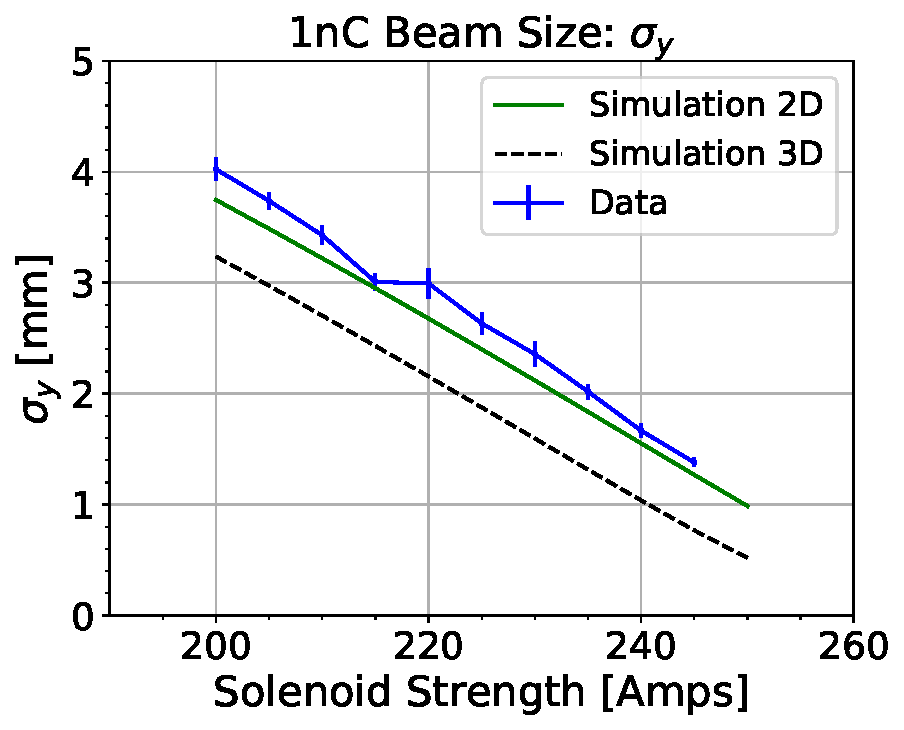
\includegraphics[width=0.45\textwidth]{images/ybeamsizes_low_charge_sol_scan_11-02-2017}\\
	
	
	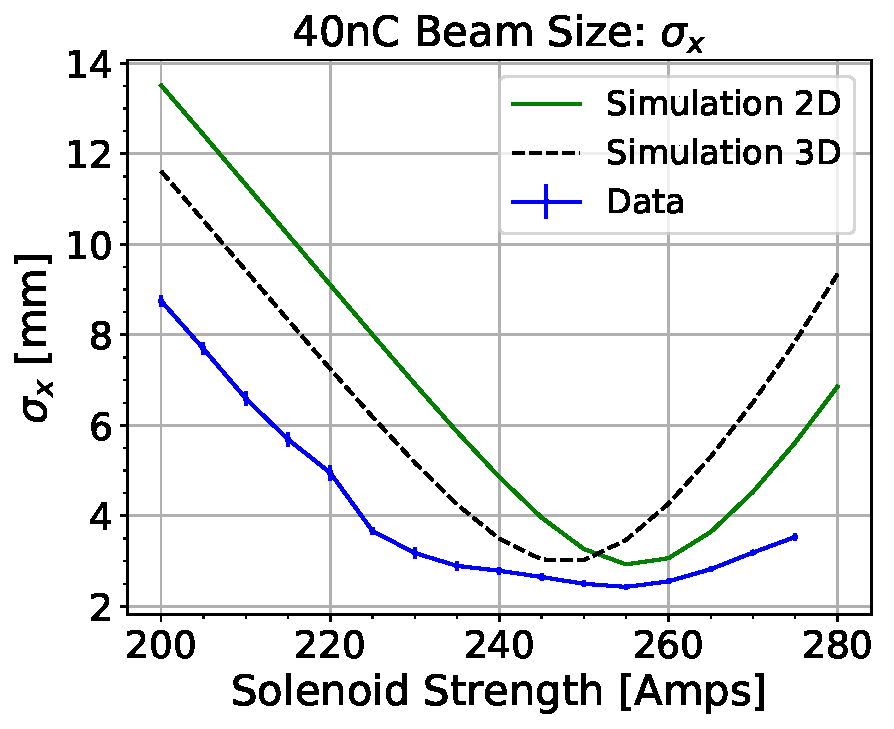
\includegraphics[width=0.45\textwidth]{images/xbeamsizes_high_charge_sol_scan_10-17-2017}%
	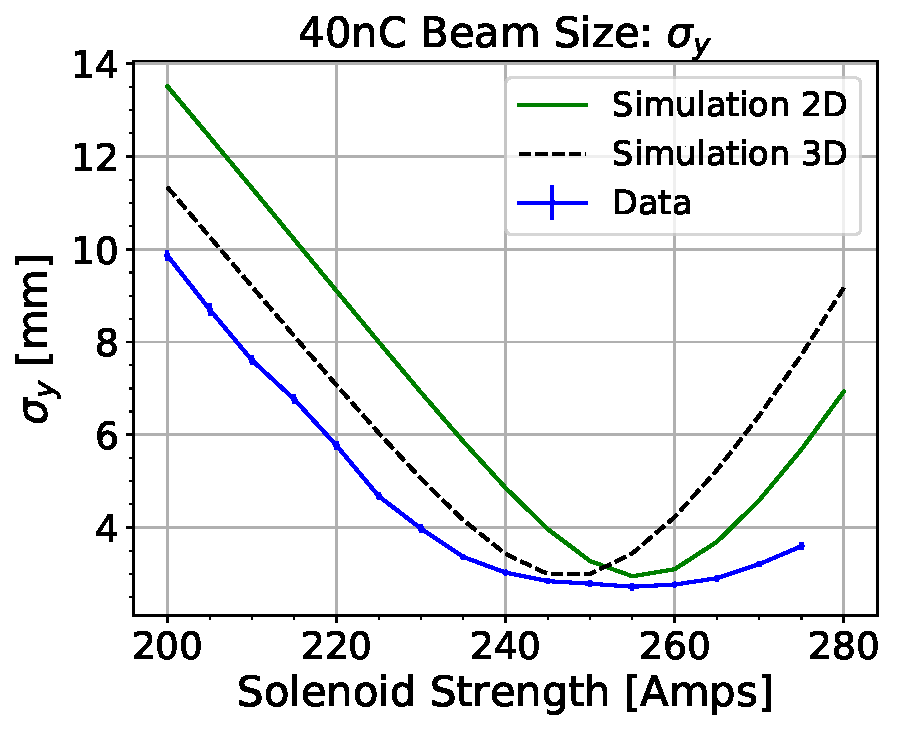
\includegraphics[width=0.45\textwidth]{images/ybeamsizes_high_charge_sol_scan_10-17-2017}
	\caption{Beam size data compared to simulations. The matching solenoid strength was varied. 
	The beam sizes were calculated using the code and methods described in Section~\ref{sec:beamsize}. 
	A rough agreement was only achieved when the gradient in the gun was lowered in the simulation.}
\label{fig:solscan}
\end{figure}


\Section{Bunch Length Measurements}\label{sec:bunchlength}

For TBA experiments, the bunch length is a key parameter.
Smaller bunch lengths result in more power out of the PETS. 
Therefore is important to be able to measure this beam characteristic 
and compare to simulations. Better understanding of the bunch length
will lead to better results in fully staged TBA.

\Subsection{Measurement Technique} 
In order to measure the bunch length, an auto-correlation scan
of the Coherent Transition Radiation (CTR) produced by the electron distribution~\cite{Happek, WBarry} was performed.
CTR is produced by the bunch when it passes through a metallic foil inserted into the beam line. 
The CTR is transported into a Michelson interferometer (MI)
where it is split and directed into two MI arms with a half-transparent pellicle~\cite{PhysRevSTAB.9.082801}. 
The CTR beams are then combined together at the exit of the MI with the variable path difference.
The resulting CTR intensity is registered with a liquid helium cooled IR Labs
bolometer~\cite{IRlabs} as a function of path difference.
The path difference is then converted into time as $\Delta \tau = 2 \Delta x$.
The resulting FWHM bunch duration is determined from the Gaussian fit of 
the interferogram; see Figure~\ref{interferogram}.
\begin{figure}
	\centering
	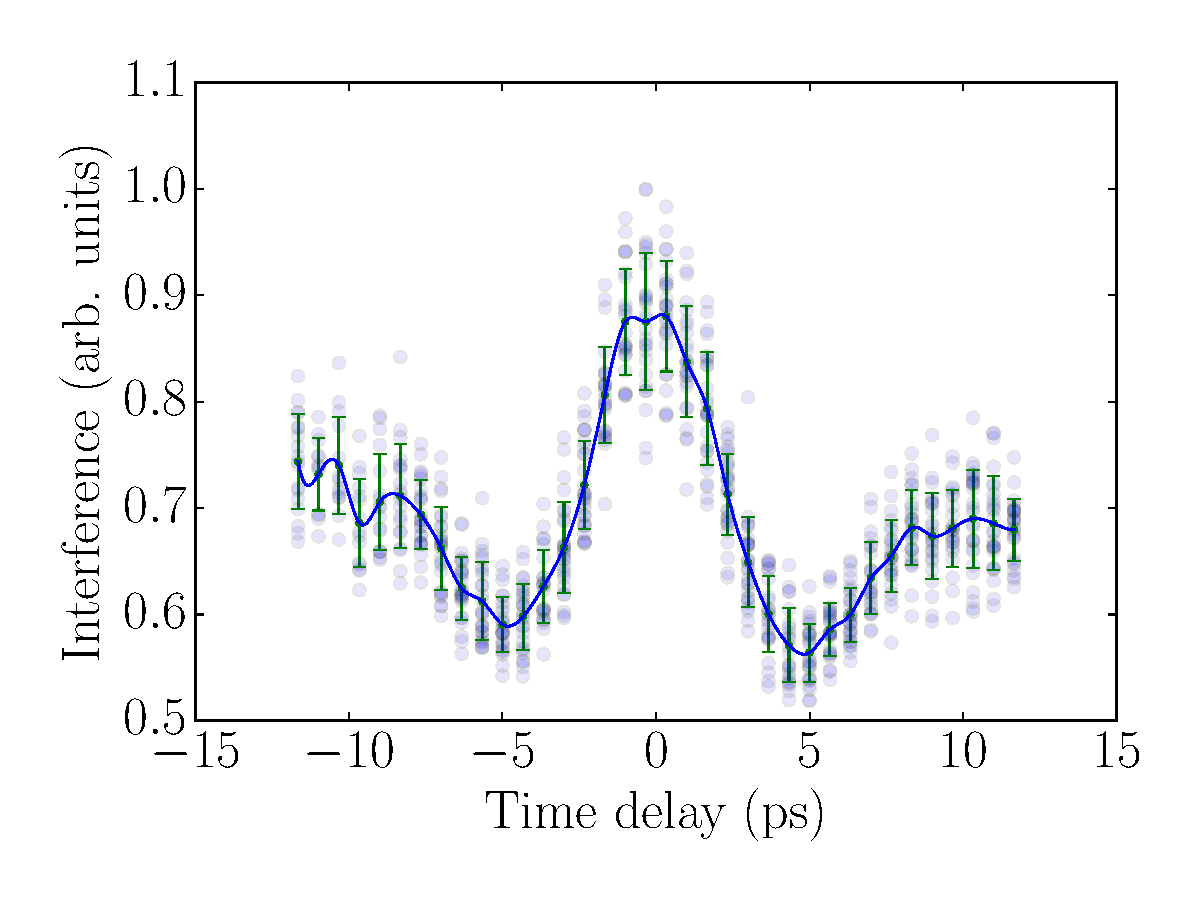
\includegraphics[width=0.75\linewidth]{images/THPMF048f1}
	\caption{An example interferogram for Q=\SI{30}{nC} and laser pulse FWHM of \SI{1.5}{ps}.}
	\label{interferogram}
\end{figure}
To alleviate the effect of charge fluctuations, 15 bolometer values for each data point were recorded.
The values were then averaged and the error bars were deduced from the data. The data points
outside of the $3\,\sigma$ bracket were considered as outliers and discarded. The resulting
interference pattern as a function of time delay in the MI is similar to that presented in Figure~\ref{interferogram}.

\begin{figure*}%[hbt]
	\centering
	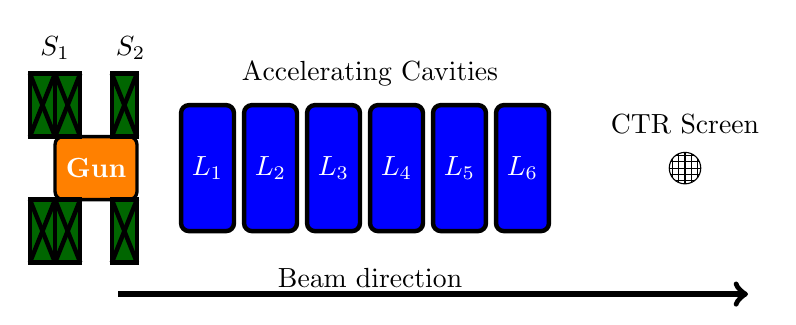
\begin{tikzpicture}[scale=0.8, text=black]
	\def \gunleft {-1.0}
\def \gunright {0.3}
\def \loneright {1.0}
\def \ltworight {2.0}
\def \lthreeright {3.0}
\def \lfourright {4.0}
\def \lfiveright {5.0}
\def \lsixright {6.0}
\def \quadone {7.5}

%Line between kicker and septum
\node[] at (4.0,-0.75) {Beam direction};
\draw[line width=0.75mm, ->] (0.0,-1.0) -- (10,-1.0);

\draw[fill=orange, very thick, rounded corners =0.1cm] (\gunleft,0.5)rectangle (\gunright,1.5) node[pos=.5, white] {\textbf{Gun}} ;
%S1
\node[] at (-1,2.9) {$S_1$};
\draw[ultra thick, fill=black!60!green] (-1.4,-0.5)rectangle  (-1.0,0.5) node[pos=.5, white] {} ;
\draw[black, ultra thick] (-1.4,-0.5) -- (-1.0,0.5);
\draw[black, ultra thick] (-1.4,0.5) -- (-1.0,-0.5);
\draw[ultra thick, fill=black!60!green] (-1.4,1.5)rectangle  (-1.0,2.5) node[pos=.5, white] {} ;
\draw[black, ultra thick] (-1.4,1.5) -- (-1.0,2.5);
\draw[black, ultra thick] (-1.4,2.5) -- (-1.0,1.5);
%S2
\draw[ultra thick, fill=black!60!green] (-1.0,-0.5)rectangle  (-0.6,0.5) node[pos=.5, white] {} ;
\draw[black, ultra thick] (-1.0,-0.5) -- (-0.6,0.5);
\draw[black, ultra thick] (-1.0,0.5) -- (-0.6,-0.5);
\draw[ultra thick, fill=black!60!green] (-1.0,1.5)rectangle  (-0.6,2.5) node[pos=.5, white] {} ;
\draw[black, ultra thick] (-1.0,1.5) -- (-0.6,2.5);
\draw[black, ultra thick] (-1.0,2.5) -- (-0.6,1.5);

%S3
\node[] at (0.2,2.9) {$S_2$};
\draw[ultra thick, fill=black!60!green] (-0.1,-0.5) rectangle  (0.3,0.5) node[pos=.5, white] {};
\draw[black, ultra thick] (-0.1,-0.5) -- (0.3,0.5);
\draw[black, ultra thick] (-0.1,0.5) -- (0.3,-0.5);
\draw[ultra thick, fill=black!60!green] (-0.1,1.5) rectangle  (0.3,2.5) node[pos=.5, white] {};
\draw[black, ultra thick] (-0.1,1.5) -- (0.3,2.5);
\draw[black, ultra thick] (-0.1,2.5) -- (0.3,1.5);
%Linac drawings 
\node[] at (4,2.5) {Accelerating Cavities};
\draw[fill=blue, ultra thick, rounded corners =0.1cm] (\loneright,0)rectangle  ({\loneright+0.84},2) node[pos=.5, white] {$L_1$} ;
\draw[fill=blue, ultra thick, rounded corners =0.1cm] (\ltworight,0)rectangle  ({\ltworight+0.84},2) node[pos=.5, white] {$L_2$};
\draw[fill=blue, ultra thick, rounded corners =0.1cm] (\lthreeright,0)rectangle ({\lthreeright+0.84},2) node[pos=.5, white] {$L_3$};
\draw[fill=blue, ultra thick, rounded corners =0.1cm] (\lfourright,0)rectangle ({\lfourright+0.84},2) node[pos=.5, white] {$L_4$};
\draw[fill=blue, ultra thick, rounded corners =0.1cm] (\lfiveright,0)rectangle ({\lfiveright+0.84},2) node[pos=.5, white] {$L_5$};
\draw[fill=blue, ultra thick, rounded corners =0.1cm] (\lsixright,0)rectangle ({\lsixright+0.84},2) node[pos=.5, white] {$L_6$};

%current optimization point
%\node[draw, fill=yellow, star, star points=5, star point ratio=0.6, minimum size=0.1cm]
%at (12.5,1.0) {$z_1$};
\node[] at (9,1.7) {CTR Screen};
\clip[draw] (9,1) circle (0.25cm);
\draw[step=1mm] (-1,-1) grid (10,10);

%Line between kicker and septum
\draw[very thick] (13.25,0.2) -- (14.5,-0.5);


%Line between septum and dipole
\draw[very thick] (15.6,-0.5) -- (16.5,-0.5);




	\end{tikzpicture}	
	\caption{Beam line layout at the AWA.}
	\label{beam line}
\end{figure*}
\Subsection{Experimental Setup}
The beam line layout is shown in Figure~\ref{beam line}. 
Bunches were allowed to propagate freely to the 
CTR screen. The only focusing elements used were solenoids $S_1$ and
$S_2$. As the bunches passed the CTR screen, light was
emitted through a window located next to the screen, 
as shown in Figure~\ref{bolo}. A slit was used to prevent
background x-rays from reaching the bolometer.
After passing the slit, the CTR propagated to the 
interferometer also shown in Figure~\ref{bolo}.   
A remotely movable stage inside the interferometer was swept, 
and the resulting combined signal fed to the bolometer. 
Periodic refilling of the helium is required when taking data in order
to keep the bolometer at \SI{4}{K}. The bolometer sensitivity knob for studies included in this work was at position ``1'' and
the gain set to 200. For the case of \SI{1}{nC} electron beams, 
the laser transverse profile was homogenized prior to the vacuum injection~\cite{PhysRevAccelBeams.20.103404}, 
using a Microlens Array~(MLA).
To produce high charge \SI{30}{nC} beams, an additional laser beam line that bypasses the homogenizer due to the losses in the 
MLA and relay optics was implemented. 
\begin{figure}
	\centering
	\begin{tikzpicture}[every node/.style={anchor=south west,inner sep=0pt},x=1mm, y=1mm,]   
	\node (fig1) at (0,0)
	{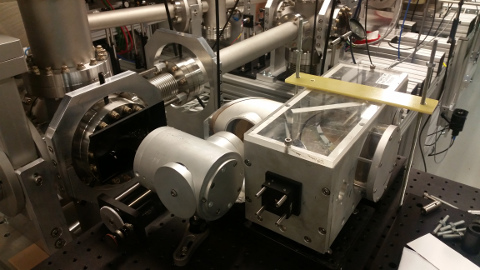
\includegraphics[width=0.5\textwidth]{images/THPMF048f3}};
	\node[fill=white, inner sep=2pt] (txt2) at (35,15) {Interferometer};
	\node[fill=white, inner sep=2pt, rotate=26] (txt2) at (18,19.5) {Slit};	
	\node[fill=white, inner sep=2pt, rotate=20] (txt2) at (13,27) {Window};
	
	\node (fig2) at (0,-50)
	{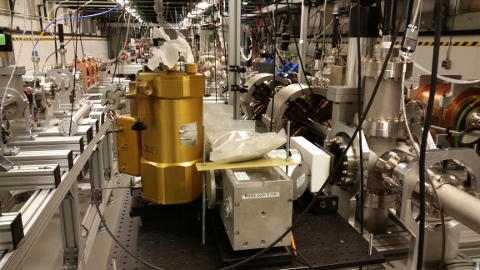
\includegraphics[width=0.5\textwidth]{images/THPMF048f4}};
	\node[fill=white, inner sep=2pt] (txt2) at (35,-42) {Interferometer};	
	\node[fill=white, inner sep=2pt] (txt2) at (55,-25) {Window};	
	\node[fill=white, inner sep=2pt] (txt2) at (22,-15) {Bolometer};
	\end{tikzpicture}
	\caption{IR labs bolometer and MI interferometer used in the experiment
		to capture CTR light as it exited a window on the beam line. }
	%\label{inter}
	%\caption{Bolometer. }
	\label{bolo}
\end{figure}


\Section{Chapter Summary}

A significant amount of preparation is 
required before the demonstration of fully staged TBA.
Since uniform bunch trains are desirable, the UV laser pulse train intensities were measured and significantly improved.
It was discovered that the UV splitters were contributing to non-uniformity in the laser intensities. 
A 16.5~\% improvement in laser pulse uniformity was achieved through the purchase and characterization of 
new splitters with a tighter tolerance on the UV coating. 
The best performing splitters were chosen, sorted and installed at the AWA, 
where they are currently in use.   

The power level (and associated fields) in the gun and linac structures must be well understood so that simulations can accurately guide optimization of the machine.
RF power measurements using the pickup probe in the gun were made and compared to previous 
measurements using the waveguide couplers. 
Measurements were also made for the linac tanks, although there exist no alternative data set to compare to at the present time, it was still possible to gain an understanding of the relative power levels in the linac cavities.  The power balance has an impact on beam dynamics.


Finally, the beam diagnostics and data processing must be understood, 
to make comparisons of experimental parameters to simulation results, 
and to quantify the success of fully staged two beam acceleration.
The procedure for energy measurements using a spectrometer was described, 
along with an example measurement, since beam energy is a critical parameter of two beam acceleration. 
Beam image analysis techniques were discussed in detail.
This includes fiducial calculation, charge selection, background subtraction, 
calculation of beam sizes, and plotting profile distributions.  All the code used is freely available on github.
An experimental measurement that used the image analysis techniques was presented. 
The experiment was a solenoid scan at the first YAG screen on the drive line.
The results informed the AWA that the gun gradient is lower than expected.
Finally, the use of CTR to perform bunch length measurements was discussed.


